%%%%
%
% ticket.sty example file for visiting cards
%
%%%%
% use the corresponding paper size for your ticket definition
\documentclass[a4paper,10pt]{letter}

% load ticket.sty with the appropriate ticket definition
\usepackage[rowmode]{ticket}

\unitlength=1mm
\hoffset=-1.9cm
\voffset=-2cm
\ticketNumbers{2}{5}
\ticketSize{98}{55} % in unitlength
\ticketDistance{3}{0}    %in unitlength

% load misc stuff
\usepackage[utf8]{inputenc}
\usepackage{lmodern}
\usepackage{fix-cm}
\usepackage{graphicx}
\usepackage{color}
\usepackage{graphics}
\usepackage{amsmath}
\usepackage{amssymb}
\usepackage{textcomp}
\usepackage{twoopt}

\usepackage{textcomp}
\usepackage{tikz}
\usetikzlibrary{shapes,arrows,positioning}

% define something
\definecolor{uni}{rgb}{.3019,.7216,.7019}
\definecolor{waterMarkColor}{rgb}{.0,.0,1.0}

% make your default ticket. \ticketdefault is somewhat like a background
% here it is empty, because we use different tickets for the front an
% the back of our card
\renewcommand{\ticketdefault}{%
}


\newcounter{questionnumber}
\setcounter{questionnumber}{1}

% now what do you like to put in your ticket
\newcommandtwoopt{\qabox}[3][][]{\ticket{%
    \put(76,51){
      \tiny\color{waterMarkColor}IACV - #1\color{black}\small\newline
    }
    \put(76.5,3){
      \tiny#2\small\newline
    }
    \put(5,55){\small%
    \framebox{
      \begin{minipage}[t][55mm][c]{85mm}%
      \vspace*{\fill}%
      #3 %\centering #3%
      \vspace*{\fill}%
      \end{minipage}%
      %
    }
    }%
 }}

\newcommand{\generateQAs}{%
\qabox[Q][\arabic{questionnumber}]{\questionA} \stepcounter{questionnumber}%
\qabox[Q][\arabic{questionnumber}]{\questionB} \stepcounter{questionnumber}%
\qabox[Q][\arabic{questionnumber}]{\questionC} \stepcounter{questionnumber}%
\qabox[Q][\arabic{questionnumber}]{\questionD} \stepcounter{questionnumber}%
\qabox[Q][\arabic{questionnumber}]{\questionE} \stepcounter{questionnumber}%
\qabox[Q][\arabic{questionnumber}]{\questionF} \stepcounter{questionnumber}%
\qabox[Q][\arabic{questionnumber}]{\questionG} \stepcounter{questionnumber}%
\qabox[Q][\arabic{questionnumber}]{\questionH} \stepcounter{questionnumber}%
\qabox[Q][\arabic{questionnumber}]{\questionI} \stepcounter{questionnumber}%
\qabox[Q][\arabic{questionnumber}]{\questionJ} \stepcounter{questionnumber}%
\qabox[A]{\answerB}%
\qabox[A]{\answerA}%
\qabox[A]{\answerD}%
\qabox[A]{\answerC}%
\qabox[A]{\answerF}%
\qabox[A]{\answerE}%
\qabox[A]{\answerH}%
\qabox[A]{\answerG}%
\qabox[A]{\answerJ}%
\qabox[A]{\answerI}%
}

\def\arraystretch{1.6}

\tikzset{%
  block/.style    = {draw, thick, rectangle, minimum height = 3em,
    minimum width = 3em},
  sum/.style      = {draw, circle, node distance = 2cm, inner sep=0pt},
  mult/.style     = {draw, circle, node distance = 2cm, inner sep=0pt},
  labelledInput/.style = {minimum height = 1em, minimum width = 1em},
  input/.style    = {coordinate},
  output/.style   = {coordinate}
}

\newcommand{\suma}{\Large$+$}
\newcommand{\multa}{\Large$\times$}

% New commands for matrices
\newcommand{\rectmat}[1]{\left[\begin{matrix}#1\end{matrix}\right]}
\newcommand{\roundmat}[1]{\left(\begin{matrix}#1\end{matrix}\right)}
\newcommand{\srectmat}[1]{\left[\begin{smallmatrix}#1\end{smallmatrix}\right]}
\newcommand{\sroundmat}[1]{\left(\begin{smallmatrix}#1\end{smallmatrix}\right)}
\setcounter{MaxMatrixCols}{20}

\begin{document}
\sffamily

\def\questionA{What is the definition of an image and how is discretized?}
\def\answerA{\textbf{Grey-scale:} Mapping from rectangular domain $\Omega = (0,w)\times(0,h)$ to a co-domain $\mathbb{R}$, s.t. $f: \mathbb{R}^2 \supset \Omega \rightarrow \mathbb{R}$.

\begin{center} \textbf{Discretization:}\end{center}
\textbf{Sampling:} Sampling $\Omega$ gives $f(i,j), 1\leq i \leq N, 1\leq j \leq M$, pixels. Low sampling $\rightarrow$ \textbf{aliasing}.

\textbf{Quantization:} Co-domain is now encoded by special value. For instance grey $0,1,\dots,255$ in bone byte.}

\def\questionB{Name some image types}
\def\answerB{\textbf{m-Dimensional:} 1D, 2D, 3D ...\\
\textbf{Vector-valued:} Co-domain in $\mathbb{R}^n$, i.e., RGB with 3 co-domain dimensions.\\
\textbf{Matrix-valued:} "Tensor". Co-domain in $\mathbb{R}^{n\times n}$, i.e., diffusion tensor MRI, f.e. voxel $3\times 3$ matrix with values.\\
\textbf{Sequences:} Videos \\}

\def\questionC{What \textbf{noise types} are there? \textbf{Describe} them:}
\def\answerC{
\textbf{Additive noise:} \underline{Most important type}. $f(i,j) = g(i,j) + n(i,j)$. Has different distributions, s.a., \textbf{uniform distribution} and \textbf{gaussian distribution}.\\
\textbf{Multiplicative noise:} Multiplicatively added, i.e., $f(i,j) = g(i,j) + g(i,j)n(i,j)$. Often appears in \textit{Radar, Ultrasound and Tomographic images}  \\
\textbf{Impulse noise:} \textbf{Unipolar} impulse noise has one degradtion. \textbf{Bipolar} impulse noise with two degrations of grey-values (low and high values for instance). \\
\textbf{Salt and Pepper noise:} Is impule noise with maximal degradtions, i.e., minimum and maximum grey-values. \\
}

\def\questionD{What are the definitions of correlation and convolution? How are they related?}
\def\answerD{Idea: Place \textbf{kernel}-box over a pixel and calculate the average.

\textbf{Correlation:} $g(i,j) = \sum\limits{k,l\in \mathbb{Z}} f(i+k, j+l) \cdot h(k,l)$. Box-smoothing has line-like artifacts, better use gaussian kernels!

\textbf{Convolution:} $g(i,j) = \sum\limits{k,l\in \mathbb{Z}} f(i-k, j-l) \cdot h(k,l) = f * h$, doing convolution is the same as "flipping" the kernel and doing correlation!}

\def\questionE{What are the boundary conditions used for correlation and convolution?}
\def\answerE{\begin{description}
    \item[zero] Standard zero-padding, dark borders
    \item[wrap] "Repeat" the whole image at the borders
    \item[clamp] Only repeat the border-pixels
    \item[mirror] "Mirror" the image at the borders
\end{description}}

\def\questionF{What are the properties of convolution?}
\def\answerF{
\begin{itemize}
    \item Commutative
    \item Associative
    \item Identity element ($\delta * h = h$)
    \item Linear (constant factor scaling and additive)
    \item Shift-invariant
\end{itemize}}

\def\questionG{How can we sharpen images?}
\def\answerG{\begin{itemize}
    \item Convolute to get a blurred image
    \item Subtract it from the original
    \item Add the result to original
\end{itemize}

\textbf{Noise:} High-frequency components - sharpening amplifies these!
}

\def\questionH{How are \textbf{MSE} and \textbf{PSNR} defined?}
\def\answerH{\textbf{Mean Square Error} $$MSE(f,g) = \frac{1}{N} \sum\limits_{n=1}^N (f_n - g_n)^2$$
\textbf{Peak signal-to-noise ratio (PSNR)} $$PSNR(f,g) = 10 \log_{10} \left(\dfrac{V^2}{MSE(f,g)}\right)$$, used to find out how good denoising is.}

\def\questionI{How does the \textbf{Bilateral Filter work}? (Idea)}
\def\answerI{To preserve edges, we average over pixels nearby with similar color. For this we have two weights: \textbf{distance} and \textbf{intensity}. \\

For distance: $N_\sigma(||x_n - x_m||)$ and for

intensity: $N_\tau(||f_n - f_m||)$, $x$ being positions, $f$ intensities.\\

We sum over the products of the two $N$ times the running $f$ and scale (down) it by the sum over the products of the two $N$.}

\def\questionJ{How does the \textbf{Non-local Means} work? (Idea):}
\def\answerJ{Images have similar patches, thus \textbf{average} using only \textbf{similar} patches.\\

Abstract approach: Use distance function $d(n,m)$ for a given square window $W_n$ to calculate kernel weights. We find the n-th pixel as the sum of the products of the weights with the intensities scaled down by the sum of the weights.\\

\textbf{It is very expensive and slow.}}

\generateQAs

%%%%%%%%%%%%%%%%%%%%%%%%%%%%%%%%%%%%%%%%%%%%%%%%%%%%%%%%%%%%%%%%%%%%%%%%%%%%%%%%%%%%%%%%%%%%%%%%%%%%%%%%%%%%%%%%%%%%%%%%
%%%%%%%%%%%%%%%%%%%%%%%%%%%%%%%%%%%%%%%%%%%%%%%%%%%%%%%%%%%%%%%%%%%%%%%%%%%%%%%%%%%%%%%%%%%%%%%%%%%%%%%%%%%%%%%%%%%%%%%%
%%%%%%%%%%%%%%%%%%%%%%%%%%%%%%%%%%%%%%%%%%%%%%%%%%%%%%%%%%%%%%%%%%%%%%%%%%%%%%%%%%%%%%%%%%%%%%%%%%%%%%%%%%%%%%%%%%%%%%%%

\def\questionA{Denoise salt and pepper noise?}
\def\answerA{Use \textbf{median filter}, since impulse noise is somewhat having \textbf{strong} outliers. They won't have a great effect if the \textbf{median} is used!}

\def\questionB{Name causes for edges and problems while detecting them}
\def\answerB{\textbf{Causes:} Reflection changes (appearance information and texture),
Depth discontinuity, Shadows, Changes in surface orientation (shape)

\textbf{Intensity as height}: \textbf{cliffs} - \textbf{gradient magnitude}\\

\textbf{Problems:} Changes in intensity often not linked to object-contours (unuseful information). Causes: Strong intensity changes (texture,shadows), No change in boundary (similar background, too dark, ...)}

\def\questionC{Name some image derivatives and their definitions:}
\def\answerC{\textbf{Continuous derivative:} 

$\partial_x f(x,y) = \lim_{\epsilon \rightarrow \infty} \dfrac{f(x + \epsilon, y) -f(x,y)}{\epsilon}$

\begin{description}
    \item[Forward diff.] $(\partial_x f)_{i,j} = \dfrac{f(i+1,j) - f(i,j)}{h_x}$
    \item[Backward diff.] $(\partial_x f)_{i,j} = \dfrac{f(i,j) - f(i-1,j)}{h_x}$
    \item[Central diff.] $(\partial_x f)_{i,j} = \dfrac{f(i+1,j) - f(i-1,j)}{2h_x}$
\end{description}}

\def\questionD{How is the gradient defined?}
\def\answerD{As the derivative in both directions: $$\nabla f = (\partial_x f, \partial_y f)$$}

\def\questionE{How is the gradient magnitude defined?}
\def\answerE{As the absolute value for the two derivatives: $$||\nabla f|| = \sqrt{(\partial_x f)^2 + (\partial_y f)^2}$$

\textbf{Properties:} Larger magnitude means stronger changes. \\

\textbf{Problems:} Noise is a problem, since \textbf{high-frequency} content is \textbf{amplified} (strong changes).}

\def\questionF{How can we improve efficiency when convoluting with derivatives?}
\def\answerF{Use the theorem: $$\partial_i (f*g) = (\partial_i f)*g = f * (\partial_i g)$$

Has predconditions on $f,g$! But advantages are: filter can be precomputed, even analytically!}

\def\questionG{Describe the Canny Edge Detector}
\def\answerG{\textbf{Non-maxima suppression idea:} Keep pixels that are on local maxima along the gradient direction (interpolation).

\textbf{Process:}

\begin{itemize}
    \item Filter with derivative of gaussian at scale $\sigma$
    \item Find magnitude and oritentation of gradient
    \item Non-maxima suppression!
    \item Linking, thresholding, two thresholds \textbf{low and max}, low starts edges and high continues them.
\end{itemize}}

\def\questionH{Explain the Scale-Space}
\def\answerH{Applying a gaussian filter with incrementing scale $\sigma$ removes detail:

\begin{itemize}
    \item Edges may shift with increasing $\sigma$
    \item Edges may merge!
    \item Edges may not split into two
    \item Multiple ways to calculate scale-spaces, \textbf{gaussian} is the "canonical" one
\end{itemize}}

\def\questionI{Name the steps of matching (features)}
\def\answerI{
\textbf{Steps for matching:}

\begin{itemize}
    \item \textbf{Detection}, identify points
    \item \textbf{Description}, extract information (feature vector)
    \item \textbf{Match}, correspondences between descriptors
\end{itemize}}

\def\questionJ{Name the goals for detectors}
\def\answerJ{\begin{itemize}
    \item \textbf{Locality}, features local, robust to occlusion and clutter
    \item \textbf{Quantity}, many for one image
    \item \textbf{Distinctiveness}, differentiate large amount of objects
    \item \textbf{Efficiency}, real-time scalability
    \item \textbf{Geometric invariance}, translation, rotation, scale!!
    \item \textbf{Photometric invariance}, intensity, brighteness, contrast, exposure
\end{itemize}}

\generateQAs

%%%%%%%%%%%%%%%%%%%%%%%%%%%%%%%%%%%%%%%%%%%%%%%%%%%%%%%%%%%%%%%%%%%%%%%%%%%%%%%%%%%%%%%%%%%%%%%%%%%%%%%%%%%%%%%%%%%%%%%%
%%%%%%%%%%%%%%%%%%%%%%%%%%%%%%%%%%%%%%%%%%%%%%%%%%%%%%%%%%%%%%%%%%%%%%%%%%%%%%%%%%%%%%%%%%%%%%%%%%%%%%%%%%%%%%%%%%%%%%%%
%%%%%%%%%%%%%%%%%%%%%%%%%%%%%%%%%%%%%%%%%%%%%%%%%%%%%%%%%%%%%%%%%%%%%%%%%%%%%%%%%%%%%%%%%%%%%%%%%%%%%%%%%%%%%%%%%%%%%%%%

\def\questionA{Characterize good features}
\def\answerA{Flat regions and edges have non-unique regions. \textbf{Corners} however, have \textbf{unique} regions where \textbf{both directions are fixed.}\\

Observe, when there is a corner, we have \textbf{points in both directions} when plotting the \textbf{distribution of data}.}

\def\questionB{What is the definition of the SVD? Describe the components!}
\def\answerB{A matrix $A \in \mathbb{R}^{m\times n}$ can be factorized in the form of $A = U \Sigma V^T$, where

\begin{itemize}
    \item $U \in \mathbb{R}^{m\times m}$ is orthogonal, $UU^T = U^T U = I_m$
    \item $V \in \mathbb{R}^{n \times n}$ is orthogonal 
    \item $\Sigma \in \mathbb{R}^{m\times n}$ is diagonal, sorted non-neg. real numbers $\sigma_1 \geq \sigma_2 \geq ... \geq 0$ and are called singular values of A.
\end{itemize}

\textbf{Singular values} are uniquely determined, $U,V$ are not. $AV = \Sigma U$ shows that, $A$ maps $V$ to $U$ scaled by $\Sigma$.}

\def\questionC{Name important properties of the SVD!}
\def\answerC{\begin{itemize}
\item \textbf{Rank of matrix:} Number of non-zero singular values
\item \textbf{Range of $A$:} Spanned by columns of $U$ where singular values non-zero (i.e. rank)
\item Columns of $V$ are eigenvectors of $A^T A$
\item Columns of $U$ are eigenvectors of $AA^T$
\item Eigenvalues of $A^T A$ and $AA^T$ are squared singular values.
\item Eigenvalues only positive or zero.
\end{itemize}}

\def\questionD{Name applications of the SVD}
\def\answerD{\begin{itemize}
    \item Can solve minimization problems
    \item PCA
    \item Linear least square homography estimation
    \item LLS for fundamental matrix estimation
\end{itemize}
}

\def\questionE{Explain what the PCA does}
\def\answerE{Intuition of SVD formalized in PCA. Goal: Characterize probability distributions of variables (e.g. to find directions with greatest variance).
\begin{itemize}
    \item Closely related to SVD
    \item Used to decorrelate data
    \item Larger singular values, higher variance, more insight
    \item high-dim. data analysis, most meaninungful lower-dimensional rep.
    \item Application: gradient measurements around pixel, analyze local orientations
\end{itemize}}

\def\questionF{Name some important definitions needed for PCA}
\def\answerF{\textbf{Expected sample value:}  $E(Z) = \sum p_iz_i$, weighted average over all measurements for $Z$.\\
\textbf{Sample variance:} $Var(Z) = \sum p_i(Z_i - E(Z))^2$, expected squared deviation from the expectation value.\\
\textbf{Sample standard deviation:} Squareroot of variance is $\sigma(Z)$\\
\textbf{Covariance of two random Variables X,Y:} $cov(X,Y) = \sum p_i(x_i - E(X))(y_i - E(Y))$.\\
\textbf{Covariance matrix:} $n\times n$ matrix for $n$ random variables:
$C(X) := (cov(X_j,X_k))_{j,k=1,\dots,n}$,\textbf{Symmetric, Diagonal is Variances, positive semi-definite}. }

\def\questionG{What is the relation between the cov. matrix and the SVD?}
\def\answerG{If $M = U \Sigma V^T$, then $M' = MV = U\Sigma$ with cov. $C' = \Sigma^T U^T U \Sigma = \Sigma^2$, i.e., cov. matrix can be made diagonal using orthogonal tranformation! The standard deviations are equal to the singular values.

\textbf{Ellipses}: Two random variables decorrelated. Ellipse given as: 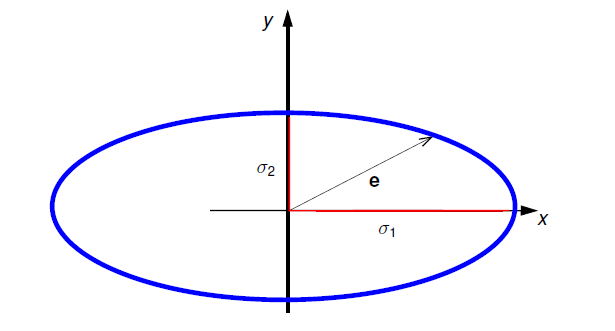
\includegraphics[width=.3\textwidth]{images/chap3/ellipse} The Radius $e$ yields $\sigma$ porjected onto the direction $\Phi$}

\def\questionH{What is the structure tensor? Describe!}
\def\answerH{\textbf{ST as gradient statistics:} Sample gradient at $\sigma$. Interested in local structure, assign weight for pixels by distance! If \textbf{gradient} has \textbf{joint distribution} for derivatives we can characterize it by:
$$\tau = G_\tau * \left[
\begin{matrix}
 (f_x^\sigma)^2 & (f_x^\sigma f_y^\sigma) \\
(f_x^\sigma f_y^\sigma) & (f_y^\sigma)^2
\end{matrix}\right]$$}

\def\questionI{What parameters do we have for the structure tensor?}
\def\answerI{For grey-scale images: \begin{itemize}
\item $\sigma > 0$, inner scale for the derivatives
\item $\tau > 0$, outer scale for the size of the window on which the derivatives are sampled on
\end{itemize}
}
\def\questionJ{What are properties on the structure tensor based on the eigenvalues?}
\def\answerJ{\begin{itemize}
    \item If one is small, the other large we have an edge (strong in one direction)
    \item If both are large we have a corner (strong in both directions)
    \item If both are small, we have a flat region (weak in both directions)
\end{itemize}}

\generateQAs

%%%%%%%%%%%%%%%%%%%%%%%%%%%%%%%%%%%%%%%%%%%%%%%%%%%%%%%%%%%%%%%%%%%%%%%%%%%%%%%%%%%%%%%%%%%%%%%%%%%%%%%%%%%%%%%%%%%%%%%%
%%%%%%%%%%%%%%%%%%%%%%%%%%%%%%%%%%%%%%%%%%%%%%%%%%%%%%%%%%%%%%%%%%%%%%%%%%%%%%%%%%%%%%%%%%%%%%%%%%%%%%%%%%%%%%%%%%%%%%%%
%%%%%%%%%%%%%%%%%%%%%%%%%%%%%%%%%%%%%%%%%%%%%%%%%%%%%%%%%%%%%%%%%%%%%%%%%%%%%%%%%%%%%%%%%%%%%%%%%%%%%%%%%%%%%%%%%%%%%%%%

\def\questionA{What is a cornerness response function?}
\def\answerA{Tells if a point looks like a corner:

\begin{itemize}
    \item Shi and Tomasi, 1994: $\lambda_2$ smaller is used
    \item Harrise 1988, Foerstner 1986: using $\det(\tau) - \mathcal{K} trace(\tau)^2 = \lambda_1 \lambda_2 - \mathcal{K}(\lambda_1+\lambda_2)^2$
\end{itemize}}

\def\questionB{What is pattern matching?}
 \def\answerB{Given a pattern, we want to find it in the image. \\
 
 \textbf{Problems:} Same as with edge detection, intensity changes, textures and so on..}

\def\questionC{What is the SSD?}
\def\answerC{The sum of squared differences: $$E_{SSD}(f,g) = \sum_i^W\sum_j^H (f(i,j)-g(i,j))^2$$, the smaller the difference the better the match.}

\def\questionD{Name properties as patch comparison metric for the SSD:}
\def\answerD{\begin{tabular}{lr}
    Fast & yes \\
    \hline    
    Invariant to translation & yes \\
    Invariant to rotation & no \\
    Invariant to scaling & no \\
    \hline
    invariant to contrast/brightness changes & No
\end{tabular}}

\def\questionE{What is the NCC?}
\def\answerE{The normalized cross-correlation: $$E_{NCC}(f,g) = \dfrac{cov(f,g)}{\sigma(f)\sigma(g)}$$, works better than SSD, but is slower. Larger values are better, the range goes from $[-1,1]$.}

\def\questionF{Name properties as patch comparison metric for the NCC:}
\def\answerF{\begin{tabular}{lr}
    Fast & no \\
    \hline    
    Invariant to translation & yes \\
    Invariant to rotation & no \\
    Invariant to scaling & no \\
    \hline
    invariant to contrast/brightness changes & yes
\end{tabular}}

\def\questionG{What is the idea behind Autocorrelation?}
\def\answerG{Displace a patch just slightly and check the two patches using SSD. It gives an idea about the stability of a patch. $$E_{AC} (f,u) = \sum_i w(p_i)(f(p_i+u)-f(p_i))^2$$}

\def\questionH{How do hybrid images work? What was Fouriers idea?}
\def\answerH{High-frequency components of one image, combined with low-frequency components of another image. The further the distance, we can only see the low frequency components.\\

\textbf{Fouriers idea:} Univariate function can be written as weighted sum of sines and cosines.}

\def\questionI{What is the definition of waves in 2D?}
\def\answerI{$f(x,y) = r \cos(2\pi (\omega_x x + \omega_y y) + \phi)$, $\omega = [\omega_x \omega_y]$ being the \textbf{wave number}, $f = |\omega|_2$ the frequency, $\omega /f$ the direction of the wave and $\phi$ the phase, $r$ the amplitude.\\

\textbf{Complex elementary wave}: For $\omega = [\omega_x \omega_y]$, $W_\omega (p) = e^{2\pi i (\omega p)} = \cos(2\pi(\omega p)) + i \sin(2\pi (\omega p))$, with phase zero, amp. one.}

\def\questionJ{Whats the central idea behind the fourier transform?}
\def\answerJ{\begin{align*}
    f(p) & = \int_{\mathbb{R}^2} \hat{f}(\omega) W_\omega (p) d\omega \\
    & = \int_{\mathbb{R}}\int_{\mathbb{R}} \hat{f} (\omega_x, \omega_y) e^{2\pi i(\omega_x x + \omega_y y)} d\omega_x d\omega_y
\end{align*}, is the inverse transform, we can get back to images
\begin{itemize}
    \item Sum of signals, is sum of fourier transforms
    \item rid of imag. part: adding it with it's conjugate
    \item Noise amplifies large frequencies
    \item Cutting some section is similar to blurring (Low-pass)
    \item Phase is more important for how a picture looks like
\end{itemize}}

\generateQAs

%%%%%%%%%%%%%%%%%%%%%%%%%%%%%%%%%%%%%%%%%%%%%%%%%%%%%%%%%%%%%%%%%%%%%%%%%%%%%%%%%%%%%%%%%%%%%%%%%%%%%%%%%%%%%%%%%%%%%%%%
%%%%%%%%%%%%%%%%%%%%%%%%%%%%%%%%%%%%%%%%%%%%%%%%%%%%%%%%%%%%%%%%%%%%%%%%%%%%%%%%%%%%%%%%%%%%%%%%%%%%%%%%%%%%%%%%%%%%%%%%
%%%%%%%%%%%%%%%%%%%%%%%%%%%%%%%%%%%%%%%%%%%%%%%%%%%%%%%%%%%%%%%%%%%%%%%%%%%%%%%%%%%%%%%%%%%%%%%%%%%%%%%%%%%%%%%%%%%%%%%%

\def\questionA{What is the definition of the fourier coefficient?}
\def\answerA{\begin{align*}
    \hat{f}(\omega) & = (f,W_\omega)_{\mathbb{C}}\\
    & = \int_{\mathbb{R}^2} f(p) \overline{W}_\omega(p) dp \\
    & = \int_{\mathbb{R}}\int_{\mathbb{R}} f(x,y) e^{-2\pi i(\omega_x x + \omega_y y)} dx dy
\end{align*}}

\def\questionB{Whats the shift - and convolution theorem?}
\def\answerB{\textbf{Shift:} $e^{2\pi i \omega p} e^{-2\pi i \omega p_0} = e^{2\pi i \omega (p-p_0)}$ \\

\textbf{Convolution}: $\widehat{f*g} = \hat{f}\hat{g}$}

\def\questionC{What is the relation between gaussians and the foruiert transform?}
\def\answerC{The \textbf{FT} of a gaussian is a gaussian-like function. When looking at the image, one can see that it corresponds to a low-pass filter.

\begin{itemize}
    \item Low-pass: gaussian
    \item High-pass: Impulse minus gaussian
    \item Band-pass: Difference of gaussians
\end{itemize}}

\def\questionD{What is the relation between derivatives and the Fourier transform?}
\def\answerD{Taking derivatives amplifies high frequencies, higher frequency and derivative order, higher amplification.

\begin{align*}
    \partial_x^n\partial_y^m f(p) & = \int_{\mathbb{R}}\int_{\mathbb{R}} \hat{f}(\omega) \partial_x^n\partial_y^m[e^{2\pi i(\omega_x x + \omega_y y)}] dx dy \\
    & = \int_{\mathbb{R}^2} (2\pi i \omega_x)^n (2\pi i \omega_y)^m \hat{f}(\omega) W_\omega (p) dp \\
 \hat{\partial_x^n\partial_y^m} f(\omega) & = (2\pi i \omega_x)^n (2\pi i \omega_y)^m \hat{f}(\omega)
\end{align*}}

\def\questionE{Name the important properties of the foruier transform}
\def\answerE{\begin{itemize}
    \item Linearity: Constant factor and additive
    \item Rotation invariant: Rotation of $f$ means rotation of $\hat{f}$ (same angle)
    \item Shift theorem
    \item Convolution theorem
    \item Derivatives
\end{itemize}}

\def\questionF{State the sampling theorem? How does it relate to downsampling?}
\def\answerF{\textbf{Sampling theorem:} $f$ band-limited, i.e., highest frequency $W$ exists with $\hat{f} (\omega) = 0$ if $|\omega|_2 > W$. The sampling rate has to be twice as high.

For sampling distance $h$ this means $h < h_{max} = 1/2W$.

\textbf{Downsampling:} Depending on the highest frequency in the image, at a certain point we get aliasing. Downsampling means reducing sampling distance $h$, reducing nyquist frequency as well.

\textbf{Solution:} Band-limit signal further before down sampling.}

\def\questionG{Explain what the gaussian pyramid is}
\def\answerG{Gaussian prefiltering: blur $\rightarrow$ downsample $\rightarrow$ blur $\rightarrow \dots$.

\textbf{Gaussian pyramid:} Represent $N\times N$ image as subimages of powers of 2 resulting in a pyramid:

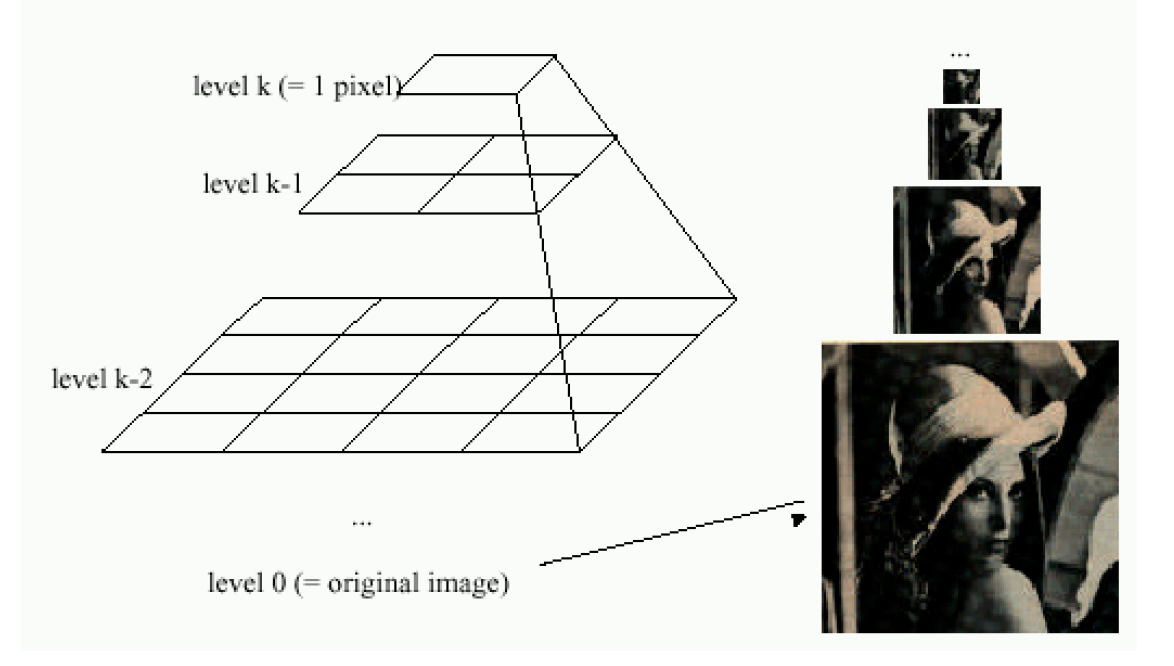
\includegraphics[width=.7\textwidth]{images/chap4/gaus_pyra}

For this we have approx. $4/3$ storage space requirement.}

\def\questionH{Explain the Laplacian Pyramid}
\def\answerH{Only store high-frequency content, instead of the full-image at subsequent levels (i.e. the DoG at each level)}

\def\questionI{Name goals of for image features from Scale-Invariant Keypoints and their applications:}
\def\answerI{\textbf{Goals:} \begin{itemize}
    \item Detect features in images (mainly corners)
    \item Detailed descriptor, as unique as possible
    \item Invariance in location, scale and orientation
\end{itemize}

\textbf{Applications:} \begin{itemize}
    \item Find sparse correspondences between images
    \item Estimate global rotations (stereo geometry, homographies, parametric transformations)
    \item Tracking, Structure from Motion
    \item Object detection, recognition
\end{itemize}}

\def\questionJ{What is the process behind SIFT?}
\def\answerJ{\textbf{Step 1:} Detect characteristic feature points.

\textit{Based on Gauss. scale-space using DoG; Extrema provide location and scale}

\textbf{Step 2:} Accurate localisation of key points

\textit{Subpixel refinement fitting quadratic functions; Discard points with high ration between principal curvatures}

\textbf{Step 3:} Assignment of dominant orientations

\textit{Histogram of gradients in local neighborhood; Refines orientation, fitting quadratic functions.}

\textbf{Step 4:} Computation of a suitable key point descriptor

\textit{Unit vector based on accumulated histograms of gradients; compensated by location, scale and dominant orientation}}

\generateQAs

%%%%%%%%%%%%%%%%%%%%%%%%%%%%%%%%%%%%%%%%%%%%%%%%%%%%%%%%%%%%%%%%%%%%%%%%%%%%%%%%%%%%%%%%%%%%%%%%%%%%%%%%%%%%%%%%%%%%%%%%
%%%%%%%%%%%%%%%%%%%%%%%%%%%%%%%%%%%%%%%%%%%%%%%%%%%%%%%%%%%%%%%%%%%%%%%%%%%%%%%%%%%%%%%%%%%%%%%%%%%%%%%%%%%%%%%%%%%%%%%%
%%%%%%%%%%%%%%%%%%%%%%%%%%%%%%%%%%%%%%%%%%%%%%%%%%%%%%%%%%%%%%%%%%%%%%%%%%%%%%%%%%%%%%%%%%%%%%%%%%%%%%%%%%%%%%%%%%%%%%%%

\def\questionA{How can we detect characteristic feature points (Step 1)?}
\def\answerA{\textbf{Idea:} Feature is strongest detector response in a scale, search for max. across scales for \textbf{scale invariance}.

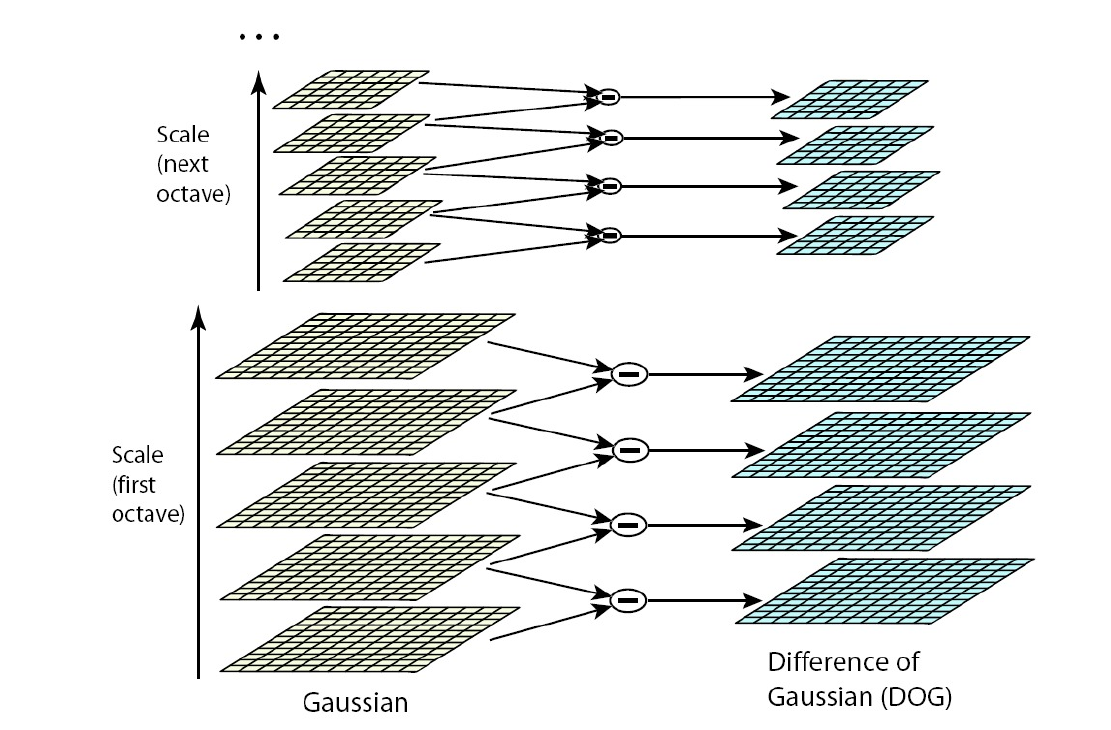
\includegraphics[width=.5\textwidth]{images/chap5/sift_DOG}

\textbf{Detection:} Filters "detect" shapes similar to their own, i.e., the LoG finds \textbf{BLOBS}.}

\def\questionB{Name properties of SIFT Step 1:}
\def\answerB{\begin{itemize}
    \item DoG is approx. of LoG, $\sigma^2 \Delta G_\sigma$ being the NLoG
    \item Factor $\sigma^2$ req. for true \textbf{scale invariance}
    \item Structures appear and vanish (bandpass behavior)
    \item At \textbf{characteristic scale} of feature, magnitude of NLoG takes extrema (min. or max.)
    \item Computing extrema in scale and space provides \textbf{location} and \textbf{scale} of features
    \item Simple case: extrema of NLoG can be found by comparing with direct neighbors in scale and space (doesn't have to be this way!)
\end{itemize}}

\def\questionC{Name the steps for accurate feature localization (idea):}
\def\answerC{\textbf{Step2a}: Sub-pixel refinement, determine sub-pixel location of extremas using Taylor expansion which is a polynomial fitting. \textbf{Improves accuracy of feature locations w.r.t. scale and location}!\\

\textbf{Step2b:} Eliminate weak conditions, i.e., features below a threshold (regions with low contrast)\\

\textbf{Step2c:} Eliminate unstable features, based on \textbf{principal curvatures}, i.e., how surface bends in different directions. If smallest and largest bending have the same sign and magnitude, the extremum is stable.}

\def\questionD{How is assignment of dominant orientations done?}
\def\answerD{Using the \textbf{histogram of gradients:} 36 bins for 360°. Weight by magnitude of gradient. \textbf{Largest entries} give \textbf{dominant} orientation.\\

\textbf{Feature cloning for multiple dominant orientations:} Every entry that is within $>$ 80\% of dominant orientation is separated and sub-bin refinement is applied.}

\def\questionE{How to compute suitable key-point descriptors?}
\def\answerE{\textbf{Block of HoGs:} Rotate patch into "default" direction. Divide neighborhood into blocks and create \textbf{HoG} for each block. An example would be 4 $4\times 4$ blocks, 32 features because we have bins of size 8. SIFT uses 16 blocks.\\

\textbf{Problem:} Slight rotation may assign different bin for same gradient. \\

\textbf{Solution:} Vote for each gradient to neighboring bins and blocks based on spatial and angular distance.}

\def\questionF{Describe the SIFT Descriptor}
\def\answerF{Stored for every feature, size 128 with 8 entries for 16 block histograms, for matching FD are compared computing euclidean norm of differences.

\begin{itemize}
    \item Invariance under scaling, shift and rotation (information computed at characteristic scale by dominant orientation)
    \item Invariance under affine illumination changes (gradient is invariant for additive illumination, normailzation makes it invariant for multiplicative illumination changes)
\end{itemize}
}

\def\questionG{Whats the naive approach to transform an Image? What are the problems?}
\def\answerG{Compute location for every pixel, throw away the pixel if it isn't in the new region and copy it to $g$ if it is.

\textbf{Problems with forward splatting:} What if $\mathbf{p'}$ not on integer pixel location?

\begin{itemize}
    \item Round coordinates, putting it to the nearest pixel - result: sever aliasing, unstable
    \item Better: Distribute among neighbors with weighting kernel
    \item Keep track of per-pixel weights, normalize
    \item Called \textbf{splatting}, suffer from aliasing and blur!
\end{itemize}}

\def\questionH{How does inverse warp work?}
\def\answerH{Compute location $\mathbf{p} = T^{-1}(\mathbf{p'})$, boundary conditions apply, copy value again. Needs knowledge about the inverse map.}

\def\questionI{Define linear transformation and common linear transformations}
\def\answerI{Map which can be written as $T(\mathbf{p}) = A\mathbf{p}$, $A \in \mathbb{R}^{2\times 2}$.

\textbf{Scaling} - $A = \left[\begin{matrix}s_x & 0 \\ 0  & s_y \end{matrix}\right]$, $s_x , s_y \neq 0$ 

\textbf{Rotation} - $A = \left[\begin{matrix}\cos \Theta & -\sin \Theta \\ \sin \Theta  & \cos \Theta \end{matrix}\right]$

Compositions of $n$ linear maps $T_1, \dots, T_n$ can be written as concatenation of application in the right order $T_n(\dots(T_1(\mathbf{p})\dots ) = A_n A_{n-1} \dots A_1 \mathbf{p} = A \mathbf{p}$. Composition of linear maps is linear}

\def\questionJ{Name properties of linear maps and their relation to the SVD}
\def\answerJ{\textbf{SVD:} Can get all information about linear maps by looking at \textbf{SVD}. $A = U \Sigma V^T$, we know $A$ maps $V$ onto scaled $U$. Another interpretation: Linear trans. can be written as \textbf{rotation} $V^T$ followed by scaling $\Sigma$, followed by another \textbf{rotation} $U$.\\

\textbf{Properties:} \textit{Origin maps to origin, Lines map to lines, parallel lines remain parallel, ratios are preserved, closed under composition}!}

\generateQAs

%%%%%%%%%%%%%%%%%%%%%%%%%%%%%%%%%%%%%%%%%%%%%%%%%%%%%%%%%%%%%%%%%%%%%%%%%%%%%%%%%%%%%%%%%%%%%%%%%%%%%%%%%%%%%%%%%%%%%%%%
%%%%%%%%%%%%%%%%%%%%%%%%%%%%%%%%%%%%%%%%%%%%%%%%%%%%%%%%%%%%%%%%%%%%%%%%%%%%%%%%%%%%%%%%%%%%%%%%%%%%%%%%%%%%%%%%%%%%%%%%
%%%%%%%%%%%%%%%%%%%%%%%%%%%%%%%%%%%%%%%%%%%%%%%%%%%%%%%%%%%%%%%%%%%%%%%%%%%%%%%%%%%%%%%%%%%%%%%%%%%%%%%%%%%%%%%%%%%%%%%%

\def\questionA{What is the definition of an affine transformation? What are its properties?}
\def\answerA{Translation missing in linear trans.: $T(x) = Ax + \mathbf{t}$ affine.\\
\textbf{Properties:} \textit{Origin is not mapping to origin}\\

\begin{itemize}
    \item \textbf{Translation} - $A = I_2$, \textbf{2 DoF}
    \item \textbf{Euclidean (rigid motion)} - $A$ pure rotation, \textbf{3 DoF} $t, \Phi$)
    \item \textbf{Similarity} - $A = sR$, \textbf{3 DoF} from before + 1 from scaling, i.e., \textbf{4 DoF!}
    \item \textbf{Area Preserving} - $det(A)  = 1$, areas stay the same, \textbf{5 DoF!}
\end{itemize}}

\def\questionB{How can we make coordinates homogeneous?}
\def\answerB{Make coordinates \textbf{homogenous} by adding a coordinate. Points on line $[wx \ wy \ w]^T$ are identified, equality holds by scaling factor $w$.

Affine maps: $T(\mathbf{p}) = A \mathbf{p} + \mathbf{t}$\\
Homogenous: $\widehat{T(\mathbf{p})} = \left[\begin{matrix}
    A & \mathbf{t} \\
    0 & 1
\end{matrix}\right]\left[\begin{matrix}
    \mathbf{p}\\
    1
\end{matrix}\right]$

\textbf{Two new parameters}: $b$ which is a two row vector. The map is called homography (projective transformation or planar perspective map).}

\def\questionC{How does the special case Homography influence a point?}
\def\answerC{$H = \left[\begin{matrix}
1 & 0 & 0 \\ 0 & 1 & 0 \\ -\frac{1}{f} & 0 & 1 
\end{matrix}\right]$, with $f \neq 0$. Then applied to a point, the image of $[x \ y]^T$ is $\left[ \begin{matrix}x \\ y \\ -\frac{x}{f+1}\end{matrix} \right] \approx
\left[ \begin{matrix}\frac{fx}{f-x} \\ \frac{fy}{f-x}\end{matrix} \right]$, if $x = f$, denominator $= 0$ hence point at infinity}

\def\questionD{What can you say about lines parallel to y-axis for the special case Homography?}
\def\answerD{$t \in \mathbb{R}$ and $x_0$ constant, then for $[x_0 \ t \ 1]^T$, mapping is $\left[ \begin{matrix}\frac{fx_0}{f-x_0} \\ \frac{ft}{f-x_0}\end{matrix} \right]$, so we get again vertical lines. But the x-coord. changes non linearly, i.e. the distances between two vertical lines may differ!}

\def\questionE{What can you say about horizontal lines for the special case Homography?}
\def\answerE{$[t \ y_0 \ 1 ]^T, t \in \mathbb{R}$, we get $\left[ \begin{matrix}\frac{ft}{f-t} \\ \frac{fy_0}{f-t}\end{matrix} \right]$, with $t \rightarrow \infty$, we get $[-f \ 0]^T$, a point at infinity in x-direction (vanishing point)}

\def\questionF{What happens if the special case homography is slightly altered?}
\def\answerF{$H = \left[\begin{matrix}
1 & 0 & 0 \\ 0 & 1 & 0 \\ -\frac{1}{f_x} & -\frac{1}{f_y} & 1 
\end{matrix}\right], f \neq 0$, vertical lines are now not vertical but intersect a vanishing point as  well, since we get for a point $\left[\begin{matrix}
-\frac{f_x f_y x}{f_y x + f_x y - f_x f_y} \\ -\frac{f_x f_y y}{f_y x + f_x y - f_x f_y}
\end{matrix}\right]$}

\def\questionG{What happens if the homography includes a translation?}
\def\answerG{
$H = \left[\begin{matrix}
1 & 0 & t_1 \\ 0 & 1 & t_2 \\ -\frac{1}{f_x} & 0 & 1 
\end{matrix}\right], f \neq 0$ for a point we get $\left[\begin{matrix}
-\frac{fx + ft_1}{f - x} \\ -\frac{fy + ft_2}{f-x}
\end{matrix}\right]$}

\def\questionH{Can you summarize the important facts about coordinate transformations?}
\def\answerH{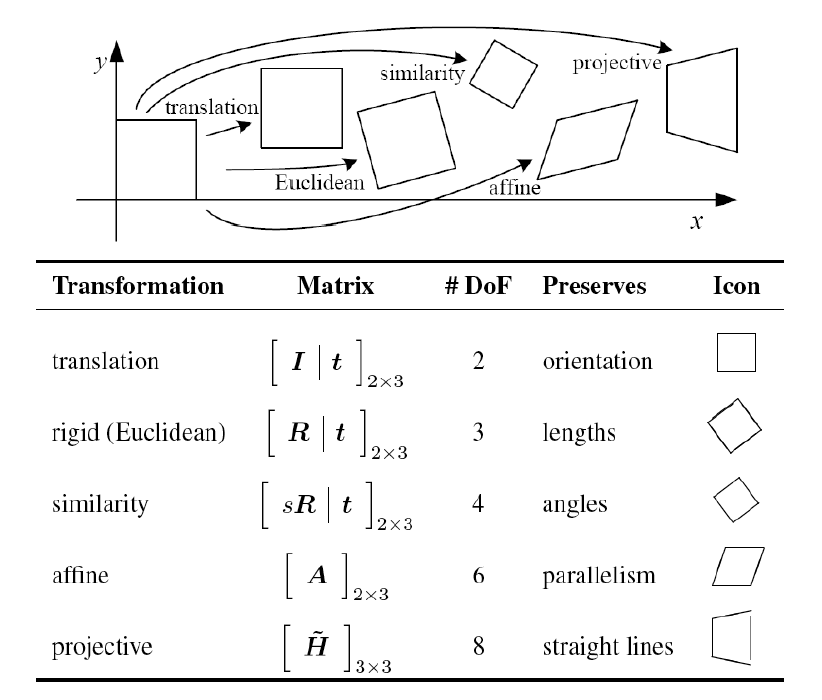
\includegraphics[width=.6\textwidth]{images/chap5/summ_coord_trans}}

\def\questionI{What's the idea behind model fitting using least squares?}
\def\answerI{Estimate $H$ using correspondences (\textbf{8 Degrees of Freedom}) \\

\textbf{Problem:} $H$ only correct up to scaling factor, need to minimize error.\\

Get two equations from each correspondence and create a linear system.

\begin{itemize}
    \item \textbf{Problem:} Overfitting/Overdetermining by having more equations than variables
    \item 2 times correspondences equations for $8$ unknowns..
    \item Frequent problem in science!
\end{itemize}}

\def\questionJ{What is the linear system for homography estimation?}
\def\answerJ{$\left[\begin{matrix}
& & & & \vdots & & & \\
-x_i & -y_i & -1 & 0 & 0 & 0 & \frac{x'_i}{w'_i}x_i & \frac{x'_i}{w'_i} y_i \\
0 & 0 & 0 & -x_i & -y_i & -1 & \frac{y'_i}{w'_i}x_i & \frac{y'_i}{w'_i} y_i \\
& & & & \vdots & & &
\end{matrix}\right]\left[
\begin{matrix}
h_{11} \\h_{12} \\h_{13} \\h_{21} \\h_{22} \\h_{23} \\h_{31} \\h_{32}
\end{matrix}\right] = \left[
\begin{matrix}
\vdots \\ -\frac{x'_i}{w'_i} \\ -\frac{y'_i}{w'_i} \\ \vdots
\end{matrix}\right]
$}

\generateQAs

%%%%%%%%%%%%%%%%%%%%%%%%%%%%%%%%%%%%%%%%%%%%%%%%%%%%%%%%%%%%%%%%%%%%%%%%%%%%%%%%%%%%%%%%%%%%%%%%%%%%%%%%%%%%%%%%%%%%%%%%
%%%%%%%%%%%%%%%%%%%%%%%%%%%%%%%%%%%%%%%%%%%%%%%%%%%%%%%%%%%%%%%%%%%%%%%%%%%%%%%%%%%%%%%%%%%%%%%%%%%%%%%%%%%%%%%%%%%%%%%%
%%%%%%%%%%%%%%%%%%%%%%%%%%%%%%%%%%%%%%%%%%%%%%%%%%%%%%%%%%%%%%%%%%%%%%%%%%%%%%%%%%%%%%%%%%%%%%%%%%%%%%%%%%%%%%%%%%%%%%%%

\def\questionA{How can we solve the linear system for homography estimation?}
\def\answerA{Using least-squares, minimizing: $\hat{x} = \mathrm{argmin}_{x\in \mathbb{R}^n} \frac{1}{2} ||Ax - b||^2$ for which we have the normal equation $A^T (A\hat{x} -b ) = 0 \leftrightarrow A^T A\hat{x} = A^T b$ (same result using analytic approach).\\

Solution to the normal equations can be found using SVD, since $A^T A$ has an inverse: $$\Sigma^2 V^T \hat{x} = \Sigma U^T b$$, due to left-inverse for $\Sigma$ we get $\hat{x} = V \Sigma^+ U^T b$ and $A^+ = V \Sigma^+ U^T$ the pseudo-inverse of $A$}

\def\questionB{What is the approach to weighted least squares?}
\def\answerB{Add weights $\sqrt{w_i}$ to the correspondences. Solution is same as before..}

\def\questionC{Whats the approach of RANSAC?}
\def\answerC{\textbf{RANdom SAmple Consensus:} \begin{itemize}
    \item {Repeat $N$ times
    \begin{itemize}
        \item Select random subset of samples
        \item Compute model
        \item Compute error between samples and model
        \item Count \textbf{inliers} by using \textbf{fixed threshold}
    \end{itemize}        
    }
    \item Refit model using largest inlier set found during the $N$ iterations
\end{itemize}}

\def\questionD{Describe the parameters of RANSAC}
\def\answerD{\textbf{1: Num samples:} Choose minimum, since
\begin{itemize}
    \item Faster fits, more iterations in same amount of time, More likely to randomly select only inliers,\textbf{Tradeoff:} Initialization may not be good for minimal sample size
\end{itemize}

\textbf{2: Threshold:} Choose with 95\% probability for an inlier to stay below threshold.\\
\textbf{3: Number $N$ of hypothesis trials:} 

Choose $N$ with $p$ so that one random sample is free from outliers. Given \textbf{percentage of outliers in the data $e$} we have $N = \frac{\log(1-p)}{\log(1-(1-e)^s)}$

Higher $s$ - faster $N$ grows in relation to the outlier amount in percent. \textbf{Works well for ratios less than 50\%}!}

\def\questionE{What is the adaptive approach/solution to RANSAC?}
\def\answerE{Problem: $e$ is unknown, need to estimate: Start with $count = 0, e= 1$ and as long as $N > count$ \begin{itemize}
    \item Perform RANSAC as usual
    \item $e \leftarrow \mathrm{min} (e , 1 - \frac{numInliers}{numPoints})$
    \item $N \leftarrow \frac{\log(1-p)}{\log(1-(1-e)^s)}$
    \item $count \leftarrow count + 1$
\end{itemize} , i.e., we update $e$ if we find a better value of $e$ out of the inliers and point amount we look at, then $N$ can be updated.}

\def\questionF{How does RANSAC work on Homography estimation?}
\def\answerF{Correspondences agree what $H$ looks like, small outlier amount does not agree.

Approach: \begin{itemize}
    \item Define max number of iterations, otherwise same as adaptive approach
    \item \textbf{In each iteration}: Select 4 correspondences randomly
    \item Compute $H$
    \item Compute error $\epsilon$ for $H$ and correspondences
    \item If the new inliers are more than previously replace everything (also $e$ and $N$ according to adaptive approach)
\end{itemize}}

\def\questionG{State the PROs and CONs of RANSAC}
\def\answerG{
\begin{itemize}
    \item[+] Simple/general
    \item[+] Many applications 
    \item[+] Works well in practice
    \item[-] Several parameters
    \item[-] Not deterministic
    \item[-] Iterative with unknown number $N$
    \item[-] Bad for low inlier ratios
    \item[-] Not always good initialization based on minimum number of samples
\end{itemize}}

\def\questionH{What is the idea behind the Hough Transform?}
\def\answerH{
\begin{itemize}
    \item \textbf{Voting Scheme} for fitting low-parameter models
    \item Detect \textbf{simple} geometric objects, represented by \textbf{very few} parameters (lines,circles)
    \item Assumptions: Boundaries with large $|\nabla|$, Points satisfy $g(\mathbf{p}, \alpha_1, \dots, \alpha_m) = 0$, $\alpha$ parameters to be determined
    \item Object Representation: Work on space of parameters, Points in param space describe different objects in image space
    \item Voting strategy: Detect all edges, Every edge point votes for all params to satisfy the upper equation, Majority rule: parameters of most relevant object gets the most votes
\end{itemize}}

\def\questionI{What are the PROs and CONs of the Hough Transform?}
\def\answerI{\begin{itemize}
    \item \textbf{Advantages:} {\begin{itemize}
        \item No fully connected contours needed
        \item Detects all objects which fit the model
        \item Very robust
    \end{itemize}}
    \item \textbf{Disadvantages:} {\begin{itemize}
        \item Memory requirements and computational effort increases rapidly with parameters
        \item Bad parallelization..
    \end{itemize}} 
\end{itemize}
}

\def\questionJ{Properties of a single camera design with a simple thin lense?}
\def\answerJ{
\textbf{Lens focuses light onto film}: \begin{itemize}
    \item Specific distance at which objects are \textbf{in focus}
    \item Determined by \textbf{focal length}
    \item Points out of focus project to \textbf{circle of confusion}
    \item Larger \textbf{circles of confusion} cause blurr
    \item \textbf{Depth of field} - range in which image appears sharp
\end{itemize}}

\generateQAs

%%%%%%%%%%%%%%%%%%%%%%%%%%%%%%%%%%%%%%%%%%%%%%%%%%%%%%%%%%%%%%%%%%%%%%%%%%%%%%%%%%%%%%%%%%%%%%%%%%%%%%%%%%%%%%%%%%%%%%%%
%%%%%%%%%%%%%%%%%%%%%%%%%%%%%%%%%%%%%%%%%%%%%%%%%%%%%%%%%%%%%%%%%%%%%%%%%%%%%%%%%%%%%%%%%%%%%%%%%%%%%%%%%%%%%%%%%%%%%%%%
%%%%%%%%%%%%%%%%%%%%%%%%%%%%%%%%%%%%%%%%%%%%%%%%%%%%%%%%%%%%%%%%%%%%%%%%%%%%%%%%%%%%%%%%%%%%%%%%%%%%%%%%%%%%%%%%%%%%%%%%

\def\questionA{Describe the pinhole camera model and it's parameters:}
\def\answerA{\footnotesize 
\textbf{Simplified but sufficiently realistic} model of a camera system. Coordinates $(X,Y,Z)$ with origin $C$ map to $m=(x,y)$ with origin $c$.
Notations: \begin{itemize}
    \item $M$, \textbf{scene point}
    \item $C$, \textbf{focal point, optical center}, pinhole location
    \item $m$, \textbf{image point} - $I$, \textbf{image plane} - $F$, \textbf{focal plane}
    \item \textbf{optical axis:} orthogonal to image plane, passes through $C$
    \item \textbf{opical ray:} passes through $M$ and $C$
    \item $f$, \textbf{focal distance}
    \item $c$, \textbf{principal point: intersection} between image plane and optical axis
\end{itemize}}

\def\questionB{What is the geometric relation between a world coordinate and a coordinate in projective space?}
\def\answerB{$\frac{x}{X} = \frac{y}{Y} = \frac{f}{Z}$, problem non-unique, non-linear: Lift to projective space! \textbf{Pinhole projection in homogenous coordinates} is projective linear map 
$\mathbb{P}^3 \rightarrow \mathbb{P}^2$: $$\hat{m} = \left[\begin{matrix}
x \\ y \\ 1
\end{matrix}\right] =\left[\begin{matrix}
Zx \\ Zy \\ Z1
\end{matrix}\right] = \left[\begin{matrix}
fX \\ fY \\ Z
\end{matrix}\right] = \underset{P}{\underbrace{\left[\begin{matrix}
f & 0 & 0 & 0 \\ 0 & f & 0 & 0 \\ 0 & 0 & 1 & 0
\end{matrix}\right]}}
\left[\begin{matrix}
X \\ Y \\ Z \\ 1
\end{matrix}\right]$$, with $P$ being the \textbf{Projection Matrix}.}

\def\questionC{Define the extrinsic parameters for cameras}
\def\answerC{Position of WCs relative CCs. 3D transformation can be expressed by $4\times 4$ \textbf{matrices}.

\textbf{Translation:} $T = \left[\begin{smallmatrix}
1 & 0 & 0 & t_1 \\ 0 & 1 & 0 & t_2 \\ 0 & 0 & 1 & t_3 \\ 0 & 0 & 0 & 1
\end{smallmatrix}\right] = \left[ \begin{smallmatrix} I & t \\ 0 & 1 \end{smallmatrix} \right]$,

\textbf{Rotation:} $R = \left[\begin{smallmatrix}
r_{11} & r_{12} & r_{13} & 0 \\ r_{21} & r_{22} & r_{23} & 0 \\ r_{31} & r_{32} & r_{33} & 0 \\ 0 & 0 & 0 & 1
\end{smallmatrix}\right] = \left[\begin{smallmatrix} R & 0 \\ 0 & 1 \end{smallmatrix} \right]$, with $RR^T = R^T R = I_4$
} 

\def\questionD{Define the rotations for different axes in 3D world coordinates}
\def\answerD{
$R_x(\Phi) = \left[\begin{smallmatrix}
1 & 0 & 0 & 0 \\ 0 & \cos \Phi & -\sin \Phi & 0 \\ 0 & \sin \Phi & \cos \Phi & 0 \\ 0 & 0 & 0 & 1
\end{smallmatrix}\right]$

$R_y(\Phi) = \left[\begin{smallmatrix}
\cos \Phi & 0 & -\sin \Phi & 0 \\ 0 & 1 & 0 & 0 \\ \sin \Phi & 0 & \cos \Phi & 0 \\ 0 & 0 & 0 & 1
\end{smallmatrix}\right]$

$R_z(\Phi) = \left[\begin{smallmatrix}
\cos \Phi & -\sin \Phi & 0 & 0 \\ \sin \Phi & \cos \Phi & 0 & 0 \\ 0 & 0 & 1 & 0 \\ 0 & 0 & 0 & 1
\end{smallmatrix}\right]$}

\def\questionE{What are intrinsic camera parameters?}
\def\answerE{Transition from image coordinates to pixel coordinates:
\begin{itemize}
    \item Origin of the image plane can be located in another point than the \textbf{principal point}
    \item Let principal point of new coordinate system be in $(u_0, v_0)$
    \item $(u,v)$ measured in pixel units has e.g., $k,l$ pixels per meter.
\end{itemize}
$$\left[\begin{smallmatrix}u \\ v \\ 1 \end{smallmatrix} \right] = \left[\begin{smallmatrix}k & 0 & u_0 \\ 0 & l & v_0 \\ 0 & 0 & 1 \end{smallmatrix} \right]\left[\begin{smallmatrix}x \\ y \\ 1 \end{smallmatrix} \right]$$}

\def\questionF{What happens to the intrinsic parameters if we have skew?}
\def\answerF{If the coordinate system is \textbf{skewed}, i.e., v-axis has an angle $\Theta \neq 90°$ to the u-axis we get:
$$\left[\begin{smallmatrix}u \\ v \\ 1 \end{smallmatrix} \right] = \left[\begin{smallmatrix}k & -k \cot\theta & u_0 \\ 0 & l/\sin\theta & v_0 \\ 0 & 0 & 1 \end{smallmatrix} \right]\left[\begin{smallmatrix}x \\ y \\ 1 \end{smallmatrix} \right]$$

In practice skew is assumed to be $0$! Also pixel sizes $k,l$ from manufacturers can generally be trusted.}

\def\questionG{How is the intrinsic matrix combined with the projection matrix (Notation):}
\def\answerG{
$$K = \underset{H}{\underbrace{\left[\begin{smallmatrix}k & -k \cot\theta & u_0 \\ 0 & l/\sin\theta & v_0 \\ 0 & 0 & 1 \end{smallmatrix} \right]\left[\begin{smallmatrix}x \\ y \\ 1 \end{smallmatrix} \right]}} \underset{P}{\underbrace{\left[\begin{smallmatrix} f & 0 & 0 & 0 \\ 0 & f & 0 & 0 \\ 0 & 0 & 1 & 0\end{smallmatrix}\right]}} = \left[\begin{smallmatrix}kf & -kf \cot\theta & u_0  & 0\\ 0 & lf/\sin\theta & v_0 & 0 \\ 0 & 0 & 1 & 0 \end{smallmatrix} \right]$$

\textbf{Focal length $f$} usually given in physical unit (meters) and as $k,l$ (pixels per meter).

\textbf{Note:} Only depends on \textbf{products} $\alpha = kf , \beta = lf$, \textbf{magnification} of the system measured in pixels.}

\def\questionH{How is the \textbf{complete} pinhole camera model defined?}
\def\answerH{$$\left[\begin{matrix}
Zu \\ Zv \\ Z
\end{matrix}\right] = \underset{=:\Pi}{\underbrace{KTR}} \left[\begin{matrix}
X_W \\ Y_W \\ Z_W \\ 1
\end{matrix}\right]$$}

\def\questionI{How is the perspective projection matrix defined?}
\def\answerI{The \textbf{perspective projection matrix} complete describes the camera model with \textbf{11 DoF}, due to arbitrary scale factors from homgenous coordinates: $\Pi = \left[\begin{smallmatrix}
    \pi_{11} & \pi_{12} & \pi_{13} & \pi_{14} \\
    \pi_{21} & \pi_{22} & \pi_{23} & \pi_{24} \\
    \pi_{31} & \pi_{32} & \pi_{33} & \pi_{34}
\end{smallmatrix}\right]$. \\

\textbf{Simplification} with the \textbf{affine} camera model is given by $\Pi_{affine} = \left[\begin{smallmatrix}
    \pi_{11} & \pi_{12} & \pi_{13} & \pi_{14} \\
    \pi_{21} & \pi_{22} & \pi_{23} & \pi_{24} \\
    0&0&0&Z_{const}
\end{smallmatrix}\right]$, if the scene points approx. have same distance $Z_{const}$ and has \textbf{6 DoF} since the 8 parameters are not independent. The mapping \textbf{is completely linear}.}

\def\questionJ{Name properties for the geometry of projection}
\def\answerJ{\begin{itemize}
    \item \textbf{Many-to-one}: Points along ray map to same point
    \item \textbf{Points map to points}: Projection on focal plane is undefined
    \item \textbf{Lines map to lines:} Lines through focal point (visual rays) project to a point.
    \item \textbf{Convex sets in 3D map to convex sets in 2D}
\end{itemize}}

\generateQAs

%%%%%%%%%%%%%%%%%%%%%%%%%%%%%%%%%%%%%%%%%%%%%%%%%%%%%%%%%%%%%%%%%%%%%%%%%%%%%%%%%%%%%%%%%%%%%%%%%%%%%%%%%%%%%%%%%%%%%%%%
%%%%%%%%%%%%%%%%%%%%%%%%%%%%%%%%%%%%%%%%%%%%%%%%%%%%%%%%%%%%%%%%%%%%%%%%%%%%%%%%%%%%%%%%%%%%%%%%%%%%%%%%%%%%%%%%%%%%%%%%
%%%%%%%%%%%%%%%%%%%%%%%%%%%%%%%%%%%%%%%%%%%%%%%%%%%%%%%%%%%%%%%%%%%%%%%%%%%%%%%%%%%%%%%%%%%%%%%%%%%%%%%%%%%%%%%%%%%%%%%%

\def\questionA{How is a vanishing point computed, given a line in world coordinates?}
\def\answerA{\scriptsize Given line in world coordinates $Mt = \srectmat{x_0 \\ y_0 \\ z_0} + \srectmat{\alpha \\ 0 \\ 1}t$ calculate projection into homogeneous coordinates:

$$PM_t = \srectmat{f&0&0&0 \\ 0&f&0&0 \\ 0&0&1&0} \srectmat{x_0 + \alpha t \\ y_0 \\ z_0 + t \\ 1} = \srectmat{f(x_0 + \alpha t) \\ fy_0 \\ z_0 + 1} \hat{=} \srectmat{\frac{f(x_0 + \alpha t)}{z_0 + t} \\ \frac{fy_0}{z_0 + t} \\ 1}$$. To calculate the vanishing point we have to calculate the limit for $t \rightarrow \infty$:

$$\lim\limits_{t\rightarrow \infty}\srectmat{\frac{f(x_0 + \alpha t)}{z_0 + t} \\ \frac{fy_0}{z_0 + t} \\ 1} = \lim\limits_{t\rightarrow \infty}\srectmat{\frac{f\alpha t}{z_0 + t} \\ 0 \\ 1} = \lim\limits_{t\rightarrow \infty}\srectmat{\frac{f\alpha t}{t(\frac{z_0}{t} + 1)} \\ 0 \\ 1} = \srectmat{f\alpha \\ 0 \\ 1}$$}

\def\questionB{How is the horizon for a world coordinate for the ground plane computed?}
\def\answerB{\scriptsize
A line on the ground plane can be written as a line where the the y-coordinate is not change by parameter $t$:

$Mt = \srectmat{x_0 \\ y_0 \\ z_0} + \srectmat{\alpha \\ 0 \\ \beta}t$, going through the same process as before: $$m_t = \srectmat{f&0&0&0 \\ 0&f&0&0 \\ 0&0&1&0} \srectmat{x_0 + \alpha t \\ y_0 \\ z_0 + \beta t \\ 1}  \hat{=} \srectmat{\frac{f(x_0 + \alpha t)}{z_0 + \beta t} \\ \frac{fy_0}{z_0 + \beta t} \\ 1}$$

calculating the limit of $t\rightarrow \infty$, we get for the horizon:

$$\lim\limits_{t\rightarrow \infty}\srectmat{\frac{f(x_0 + \alpha t)}{z_0 + \beta t} \\ \frac{fy_0}{z_0 + \beta t} \\ 1} = \lim\limits_{t\rightarrow \infty}\srectmat{\frac{f\alpha t}{z_0 + \beta t} \\ 0 \\ 1} = \lim\limits_{t\rightarrow \infty}\srectmat{\frac{f\alpha t}{t(\frac{z_0}{t} + \beta)} \\ 0 \\ 1} = \srectmat{\frac{f\alpha}{\beta} \\ 0 \\ 1}$$}

\def\questionC{How does a translation of the camera in y-direction change the horizon?}
\def\answerC{It doesn't, a translation has no effect on the projection of the horizon.}

\def\questionD{What happens if the camera is rotate around the x-axis?}
\def\answerD{\scriptsize
Optical center fixed, camera rotated 15 degrees around X-axis. Recalculating all possible directions: $$d'(\alpha, \beta) = R_X(\Phi)d(\alpha,\beta) = \srectmat{1 & 0 & 0 & 0 \\ 0 & \cos \Phi & -\sin \Phi & 0 \\ 0 & \sin \Phi & \cos \Phi & 0 \\ 0 & 0 & 0 & 1} \srectmat{\alpha \\ 0 \\ \beta \\ 1} = \srectmat{\alpha \\ -\beta \sin\Phi \\ \beta \cos \Phi \\ 1}$$, this is only the new direction vector, we need to calculate the horizon using this direction vector, as we've done before, going through all calculations we end up at the horizon $$\srectmat{\frac{f\alpha}{\beta\cos\Phi} \\ -\frac{f\sin\Phi}{\cos\Phi} \\ 1} = \srectmat{\frac{f\alpha}{\beta\cos\Phi} \\ -f \tan \Phi \\ 1}$$. In this example the horizon \textbf{moves up} $-\tan(-15°) * f) = 0.2679 * f$ pixels.}

\def\questionE{Are homographies given when?}
\def\answerE{

\textbf{Are homographies given when} \begin{itemize}
    \item Translating cameras: Not always, objects can get in front of the scene
    \item Capturing images of a plane: Yes
    \item Rotation: Yes
\end{itemize}

\textbf{Why are planes homographies?} We can assume \textbf{WCS} is chosen, s.t. the plane is parametrized in world coordinates with $[p \ q \ 0 \ 1]^T$. Applying $PRT$ on this point we get a homography.

\textbf{Punchline 1:} Planar surfaces in 3D, reduces projection to a 2D to 2D transformation.

\textbf{Punchline 2:} Transformation is invertible!}

\def\questionF{Why does rotation of the camera result in a homography?}
\def\answerF{Let $\srectmat{u \\ v \\ 1} \hat{=} K \srectmat{X \\ Y \\ Z}$ be the primary projection. When rotated we can write $\srectmat{u' \\ v '\\ 1} \hat{=} KR \srectmat{X \\ Y \\ Z} = KRK^{-1}K \srectmat{X \\ Y \\ Z} \hat{=}  KRK^{-1} \srectmat{u \\ v \\ 1}$

$KRK^{-1}$ is the homography between images (called "conjugate relation").}

\def\questionG{What needs to be done for pinhole camera calibration?}
\def\answerG{\begin{itemize}
    \item Determine the \textbf{5 intrinsic} and \textbf{6 extrinsic} parameters
    \item Many algos proposed
    \item \textbf{Basic idea:} Investigate image of \textbf{known} size and shape
    \item Identified point corresponds to 2 constraints
    \item For 11 parameters we need 6 correspondences
    \item Considering more points, makes estimation less sensitive w.r.t. errors
\end{itemize}}

\def\questionH{What are the basic equations to pinhole camera calibration?}
\def\answerH{\scriptsize
\textbf{Input:} We have $k$ correspondences (for which we know the world to image correspondences)

\textbf{Output:} Perspective projection matrix $\Pi = \left[\begin{smallmatrix}
    \pi_{11} & \pi_{12} & \pi_{13} & \pi_{14} \\
    \pi_{21} & \pi_{22} & \pi_{23} & \pi_{24} \\
    \pi_{31} & \pi_{32} & \pi_{33} & \pi_{34}
\end{smallmatrix}\right]$, with $$\widehat{\srectmat{u^i \\ v^i}} = \srectmat{u^i \\ v^i \\ 1} \hat{=} \srectmat{Z^i u^i \\ Z^i v^i \\ Z^i} = \rectmat{\pi_{11} & \pi_{12} & \pi_{13} & \pi_{14} \\
    \pi_{21} & \pi_{22} & \pi_{23} & \pi_{24} \\
    \pi_{31} & \pi_{32} & \pi_{33} & \pi_{34}} \srectmat{X^i_w \\ Y^i_w \\ Z^i_w \\ 1}$$

\textbf{Problem}: We do not know $Z$ since we lost \textbf{DEPTH} information during projection.}

\def\questionI{What is the homogeneous linear system for pinhole camera calibration?}
\def\answerI{$\srectmat{& & & & & & \vdots & & & & & \\
-X^i_W & -Y^i_W & -Z^i_W & -1 & 0 & 0 & 0 & 0 & u^i X^i_W & u^i Y^i_W & u^i Z^i_W & u^i\\
0 & 0 & 0 & 0 & -X^i_W & -Y^i_W & -Z^i_W & -1 & v^i X^i_W & v^i Y^i_W & v^i Z^i_W & v^i\\
& & & & & & \vdots & & & & &} \newline \cdot
\srectmat{\pi_{11} \\\pi_{12} \\ \pi_{13} \\ \pi_{14} \\ \pi_{21} \\ \pi_{22} \\ \pi_{23} \\ \pi_{24} \\ \pi_{31} \\ \pi_{32} \\ \pi_{33} \\ \pi_{34}} = 0$, which can be solved using the \textbf{SVD!}}

\def\questionJ{How can you solve a homogeneous system using the SVD?}
\def\answerJ{

\textbf{Formally,} $A = U\Sigma V^T$, thus $$||Ax||^2 = (Ax,Ax) = x^T(A^T A) x = (V^Tx)^T \Sigma^2 V^T x$$

\textbf{Algorithm:} \underline{Direct linear transformation}

\begin{itemize}
    \item For $k$ correspondences, compute $2k \times 12$ matrix $A$ (set of basic equations)
    \item Compute the SVD
    \item The last column of $V$ is the entries of $\Pi$ since it corresponds to the smalles singular value!
\end{itemize}}

\generateQAs

%%%%%%%%%%%%%%%%%%%%%%%%%%%%%%%%%%%%%%%%%%%%%%%%%%%%%%%%%%%%%%%%%%%%%%%%%%%%%%%%%%%%%%%%%%%%%%%%%%%%%%%%%%%%%%%%%%%%%%%%
%%%%%%%%%%%%%%%%%%%%%%%%%%%%%%%%%%%%%%%%%%%%%%%%%%%%%%%%%%%%%%%%%%%%%%%%%%%%%%%%%%%%%%%%%%%%%%%%%%%%%%%%%%%%%%%%%%%%%%%%
%%%%%%%%%%%%%%%%%%%%%%%%%%%%%%%%%%%%%%%%%%%%%%%%%%%%%%%%%%%%%%%%%%%%%%%%%%%%%%%%%%%%%%%%%%%%%%%%%%%%%%%%%%%%%%%%%%%%%%%%

\def\questionA{What can you say about world to image correspondences? How do we get them?}
\def\answerA{For this we need a \textbf{Calibration object} with known geometry. Can be previously selected and placed, can also be already in the scene but known.

\textbf{Need to locate correspondences with subpixel precision for exact calibration!}}

\def\questionB{What are degenerate configurations?}
\def\answerB{Choice of correspondences, s.t. there is no unique solution. Even close to degenerate choices lead to unstable results. Select correspondences in general positions.

\textbf{Important degenerate} configuration is if all points lie on one plane.}

\def\questionC{What constraints can we introduced if we know the camera?}
\def\answerC{
\textbf{Useful theorem:} $\Pi , 3\times 4$ projection matrix, $a_i^T$ rows of $A$ which is formed of the left-three-columns of $\Pi$: \begin{itemize}
    \item $\Pi$ is a projection matrix iff $\det(A) \neq 0$
    \item $\Pi$ is zero-skew iff additionally $(a_1 \times a_3) \cdot (a_2 \times a_3) = 0$
    \item $\Pi$ has unit aspect ratio (square pixels) iff $(a_1 \times a_3) \cdot (a_1 \times a_3) = (a_2 \times a_3) \cdot (a_2 \times a_3)$
\end{itemize}}

\def\questionD{What are ideal points and ideal lines?}
\def\answerD{\textbf{Ideal points:} Points in $\mathbb{p}^2$ with $c = 0$ are ideal points, points at infinity.

\textbf{Normal form of a line:} $a^2 + b^2 = 1$, $[a \ b]^T$ is the normal with distance $c$ to the origin.

\textbf{Line at infinity:} $a,b = 0$ then we get $l_\infty = \srectmat{0 \\ 0 \\ 1}$
\begin{itemize}
    \item Abstract notation simplifies some calculations
    \item Some geometric relations are simpler to describe
    \item Certain special cases need not be distinguished anymore
\end{itemize}}

\def\questionE{How are lines intersected in projective coordinates?}
\def\answerE{
Let $\mathbf{l, l'}$ be two lines. Point of intersection: $\mathbf{x = l \times l'}$, $\times$ being the cross-product in $\mathbb{R}^3$.

\textbf{Cross-product:} $\mathbf{a,b} \in \mathbb{R}^3$, $\mathbf{a \times b} := [\mathbf{a}]_\times \mathbf{b} = \srectmat{a_2b_3-a_3b_2 \\ a_3b_1 - a_1b_3 \\ a_1b_2 - a_2 b_1}$, rule of thumb: \textbf{[23,31,12]}!

$[a]_\times = \srectmat{0 & -a_3 & a_2 \\ a_3 & 0 & -a_1 \\ -a_2 & a_1 & 0}$ is the anti-symmetric matrix of $\mathbf{a}$.\\
\textbf{Important rules}: \begin{itemize}
        \item $a^T(a\times b) = b^T(a \times b) = 0$
        \item $M \in \mathbb{R}^{3\times 3}$ a transformation, them $(Ma) \times (Mb) = M^{-T} (a\times b)$
    \end{itemize}
}

\def\questionF{How do we compute a line through two points?}
\def\answerF{
$\mathbf{x, x'}$ points, then $\mathbf{l = x \times x'}$ is the line that goes through both (\textbf{duality}).

\textbf{"Fun" facts:} $\mathbf{l, l'}$ both have direction $\mathbf{d}$, then their intersection is in the ideal point $\srectmat{\mathbf{d} \\ 0}$ at infinity

If $\mathbf{l}$ has direction $\mathbf{d}$, then it also intersect $\mathbf{l}_\infty$ in the ideal point.

$\mathbf{x, x'}$ ideal points, then the line that goes through both is the ideal line $\mathbf{l}_\infty$.}

\def\questionG{How can we find the image of a line for a homography?}
\def\answerG{
Suppose we are given $H$, what is the image of a line $\mathbf{l}$ under the homography?

Map two points to the homography and connect them $$\mathbf{l'} = (Hx \times Hx') = H^{-T} (x \times x') = H^{-T} \mathbf{l}$$, i.e. the inverse transpose of $H$.}

\def\questionH{How can we describe the relation of a WC on two cameras?}
\def\answerH{Using the epipolar geometry:

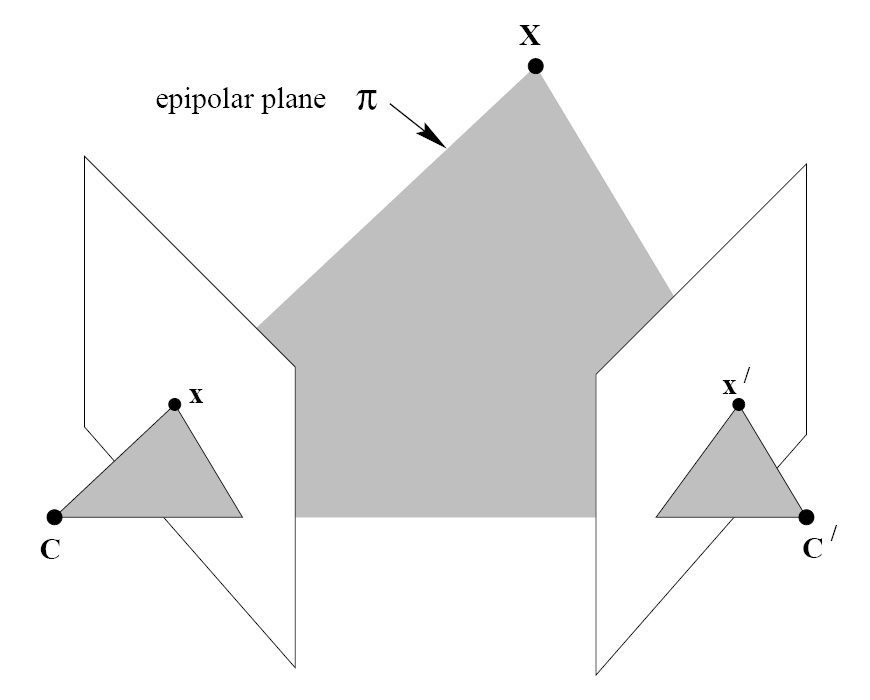
\includegraphics[width=.7\textwidth]{images/chap8/point_correspondence_geometry}}

\def\questionI{What constraints can be set upon a point in one view, knowing the correspondence in the other view?}
\def\answerI{
\textbf{Constraints on $x'$ given $x$:} \begin{itemize}
    \item $\mathbf{X}$ must lie on optic ray connecting $C$ and $\mathbf{x}$.
    \item $\mathbf{x'}$ must lie on the projection $\mathbf{l}'$ of this optic ray in $C'$
    \item This projection is called epipolar line corresponding to $\mathbf{x}$
\end{itemize}}

\def\questionJ{State properties of epipolar planes and lines}
\def\answerJ{
\begin{itemize}
    \item Baseline intersects the imageplane in epipoles $e, e'$
    \item Any plane $\Pi$ containing the baseline is an epipolar plane
    \item Intersections of $\Pi$ with the image planes are epipolar lines $l,l'$
    \item Moving a scene point $\mathbf{X}$ up or down, rotates the epipolar plane around the baseline
    \item All epipolar lines in one view, intersect at the corresponding epipole
\end{itemize}}

\generateQAs

%%%%%%%%%%%%%%%%%%%%%%%%%%%%%%%%%%%%%%%%%%%%%%%%%%%%%%%%%%%%%%%%%%%%%%%%%%%%%%%%%%%%%%%%%%%%%%%%%%%%%%%%%%%%%%%%%%%%%%%%
%%%%%%%%%%%%%%%%%%%%%%%%%%%%%%%%%%%%%%%%%%%%%%%%%%%%%%%%%%%%%%%%%%%%%%%%%%%%%%%%%%%%%%%%%%%%%%%%%%%%%%%%%%%%%%%%%%%%%%%%
%%%%%%%%%%%%%%%%%%%%%%%%%%%%%%%%%%%%%%%%%%%%%%%%%%%%%%%%%%%%%%%%%%%%%%%%%%%%%%%%%%%%%%%%%%%%%%%%%%%%%%%%%%%%%%%%%%%%%%%%

\def\questionA{How is the Fundamental Matrix defined? What are its properties?}
\def\answerA{\scriptsize \textbf{Theorem} Given $P, P'$, there exists $F \in \mathbb{R}^{3\times 3}$, s.t., $\mathbf{l}'$ for $\mathbf{x}$ is given by $\mathbf{l}' = F \mathbf{x}$, a pair of correspondences satisfies $\mathbf{x'}^T F \mathbf{x} = 0$,

$F$ is called the \textbf{Fundamental matrix} for the two views and can be estimated by correspondences alone.

\textbf{Properties:} \begin{itemize}
    \item $F$ for $(P,P')$, then $F^T$ for $(P',P)$ (\textbf{transpose correspondence equation)}
    \item The epipole $\mathbf{e'}$ is the left nullspace of $F$, i.e., $\mathbf{e'}^T F = 0$ and $F \mathbf{e} = 0$ (\textbf{all epilines contain the epipoles}), these equations \textbf{are used} to compute the epipoles once F is found
    \item $F$ has rank 2 (only the first two diagonal values are not zero)
    \item $F$ has \textbf{7 Degrees of Freedom}
\end{itemize}
}

\def\questionB{How can we compute the fundamental matrix for camera pairs?}
\def\answerB{1. Given $\mathbf{x}$ compute $\mathbf{X}_W$ which projects to $\mathbf{x}$. Using the pseudo-inverse we can find such a point using $\mathbf{X}_W = P^+ \mathbf{x}$

2. Project $\mathbf{X}_W$ into the second image using $P'$

3. Using the previously discussed property, we know that the epiline connects the epipole $\mathbf{e'}$ with $P'\mathbf{X}_W$, $$\mathbf{l'} = [\mathbf{e'}]_\times P' \mathbf{X}_W = \underset{=F}{\underbrace{[\mathbf{e'}]_\times P' P^+}} \mathbf{x}$$

4. The epipole $\mathbf{e'}$ is the projection of $P'C_w$ of the camera center of the first camera in world space, defined by $PC_W = 0$}

\def\questionC{What is the definition of the pseudo-inverse of the projection matrix?}
\def\answerC{Using the SVD: $P^+ = V \Sigma^+ U^T$, $\Sigma^+$ constructed from $\Sigma$ taking the reciprocal of the diagonal values and then transposing the matrix. For projection matrices $n < m$ and we get $\Sigma^+$ as a right-inverse of $\Sigma$, thus $$PP^+ = U\Sigma V^T V\Sigma^+ U^T = I_3$$.}

\def\questionD{What is the solution for the fundamental matrix?}
\def\answerD{$n<m$: Situation for the fundamental matrix. System is \textbf{under-determined}, infinitely many solutions. Pseudo-inverse $\hat{x} = A^+ b$ computes $Ax = b$ which minimizes \textbf{the norm of} $x$: $$\hat{x} = \mathrm{argmin}_{Ax = b} ||x||$$.
I.e., computes a minimum norm solution for $Ax = b$. The pseudo-inverse is a \textbf{right-inverse}.}

\def\questionE{What can you say about pure translational motions?}
\def\answerE{Choose parameters $P = K[I | 0], P' = K[I | t]$. Then $P^+ = [K^{-1} \ 0]^T$ and $P'P^+ = KK^{-1} = I_3$, hence the result is \textbf{independent of translation}.

Also $C' = [-t \ 1]^T$ in world coords, thus $\mathbf{e} = K[I|0] [-t | 1]^T = -K t = Kt$ and $\mathbf{e'} = K[I|t][0 \ 1]^T = Kt$ and we have $\mathbf{e} = \mathbf{e'}$.

\textbf{Horizontal motion}

Parallel to x-axis: epipole at $\mathbf{e'} = [1 \ 0 \ 0]^T$ and thus $$F = \srectmat{0 & 0 & 0\\ 0 & 0 & -1 \\ 0 & 1 & 0}$$ and the correspondence relation reduces $x' F x = 0$ to $y = y'$, along horizontal lines.
}

\def\questionF{How can we estimate F?}
\def\answerF{Given $n$ correspondences, for the $i$-th correspondence we get the constraint: 
$$0 = \mathbf{x'}_i F \mathbf{x}_i = [x'_i \ y'_i \ 1] \srectmat{f_{11} & f_{12} & f_{13} \\ f_{21} & f_{22} & f_{23} \\ f_{31} & f_{32} & f_{33}}[x_i \ y_i \ 1]$$ which resolves in the equation $x_ix'_i f_{11} + y_ix'_i f_{12} +x'_i f_{13} + x_ix'_i f_{21} + y_ix'_i f_{22} + y'_i f_{23} + x_i f_{31} + y_i f_{32} + f_{33}$, build the linear system and solve with \textbf{SVD} (rightmost column), \textbf{enforce RANK-2} and optimize using \textbf{RANSAC}!}

\def\questionG{What is projective ambiguity?}
\def\answerG{\textbf{Projective ambiguity}: Given correspondences and assuming we reconstructed $P,P'$ and some world coordinates. Given \textbf{any} homography of the world, applying it onto the world coordinates and the projections (computing new cameras), we get the \textbf{same fundamental matrices} for the new and the old projections!

I.e., both reconstructions lead to \textbf{exactly the same correspondences}. \textbf{Mathematical limit of what we can reconstruct from correspondences alone!}

This is \textbf{projective reconstruction}.}

\def\questionH{What is affine reconstruction? What is the advantage?}
\def\answerH{Parallel lines map to parallel lines, angles are not necessarily correct.. In order to do this, we need to get rid of \textbf{projective ambiguity}. One possibility is, to identify the \textbf{plane at infinity} $\pi_\infty$.

\textbf{Plane at infinity:} Can be identified, e.g., from correspondences of \textbf{three vanishing points} detected in both images. (For instance 3 sets of parallel lines).}

\def\questionI{What is metric reconstruction? What is the advantage?}
\def\answerI{Correct reconstruction \textbf{up to similarity} transformations (parallel lines and angles correct), but the scene might be scaled uniformly.

\textbf{Scaling ambiguity:} Segment with known absolute length must be identified (in both images).

In order to do \textbf{metric reconstruction}, we need to identify \textbf{absolute angles} (complex and not discussed!). Short: Find intrinsic parameters $K$, for which we need to compute the \textbf{Image of the Absolute Conic} (IAC), which can be described by $3\times 3$ symmetric matrix $\omega = (KK^T)^{-1}$. If $\omega$ is known, $K$ can be recovered by inverting $\omega$ and computing \textbf{Cholesky decomposition}. (The last part is not that important I guess).}

\def\questionJ{What are the conditions we can put on for the IAC?}
\def\answerJ{
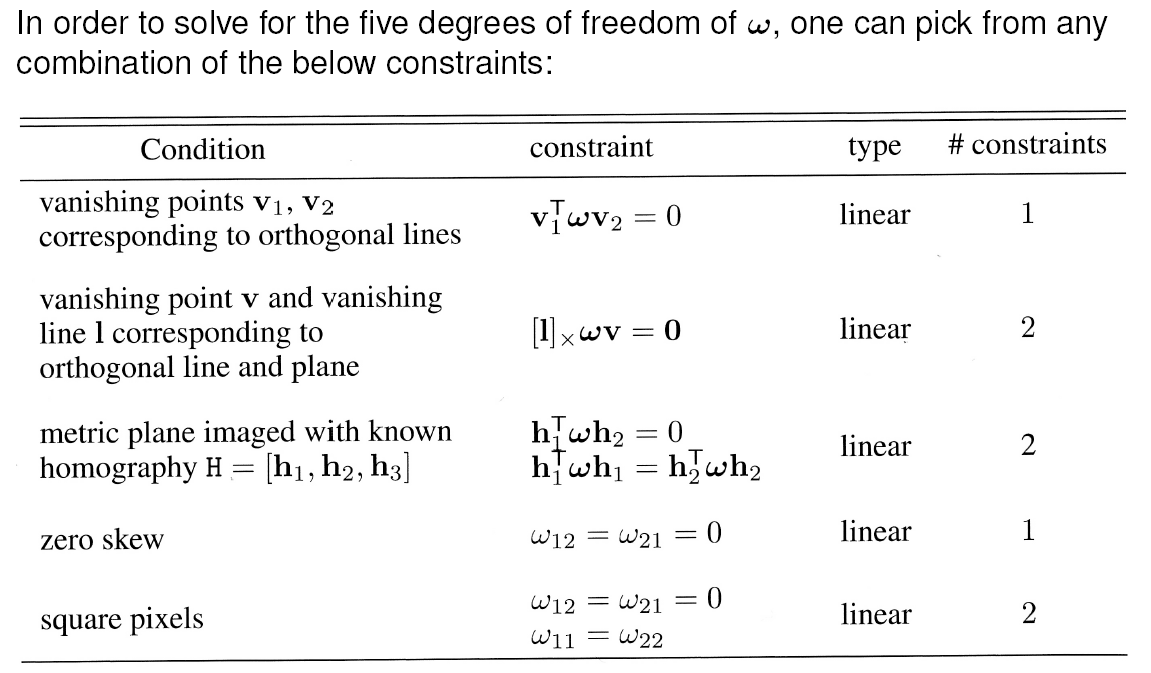
\includegraphics[width=.9\textwidth]{images/chap8/omega_conditions}}

\generateQAs

%%%%%%%%%%%%%%%%%%%%%%%%%%%%%%%%%%%%%%%%%%%%%%%%%%%%%%%%%%%%%%%%%%%%%%%%%%%%%%%%%%%%%%%%%%%%%%%%%%%%%%%%%%%%%%%%%%%%%%%%
%%%%%%%%%%%%%%%%%%%%%%%%%%%%%%%%%%%%%%%%%%%%%%%%%%%%%%%%%%%%%%%%%%%%%%%%%%%%%%%%%%%%%%%%%%%%%%%%%%%%%%%%%%%%%%%%%%%%%%%%
%%%%%%%%%%%%%%%%%%%%%%%%%%%%%%%%%%%%%%%%%%%%%%%%%%%%%%%%%%%%%%%%%%%%%%%%%%%%%%%%%%%%%%%%%%%%%%%%%%%%%%%%%%%%%%%%%%%%%%%%

\def\questionA{What is pose estimation and the essential matrix?}
\def\answerA{\scriptsize \textbf{Essential matrix:} Specialization of fundamental matrix to the pre-calibrated case where $K$ is known (hence we have \textbf{metric reconstruction}).

Under assumptions \textbf{square pixels, center of projection is center of image} we only need to calibrate the \textbf{magnification} of $K$ (focal length times pixels per meter).

\textbf{Definition:} Defined in terms of homogeneous coordinates. From a corresponding pair we get the correspondence: $K^{-1} x = \hat{x} \leftrightarrow \hat{x}' = K'^{-1} x'$.

The defining equation for $E$ is the correspondence constraint $\hat{x}'^T E \hat{x} = 0$. Thus, $E = K'^T F K$, and $E$ has rank two.

\textbf{Derivation from a pair of cameras:} Given a \textbf{normalized} camera pair $P = [I|0], P' = [R|t]$, we get for $E$: $$E = [e']_x P'P^+ = [[R|t][0 \ 0 \ 0 \ 1]^T]_\times [R|t][I \ 0]^T = [t]_\times R$$}

\def\questionB{How does triangulation work?}
\def\answerB{\scriptsize We want to find a 3D world point $PX = x$ and $P'X = x'$. Correspondence measurements usually have errors, but we can compute it (non-error free) by minimizing the \textbf{reprojection error}: $E(X) = \sum\limits_{i=1}^n ||PX - x||^2 + ||P'X - x'||^2$.

\textbf{Direct linear triangulation:} $X$ can be recovered as solution to $AX = 0$:

$$A = \srectmat{x(p^3) - p^1 \\ y(p^3) - p^2 \\ x'(p'^3) - p'^1 \\ y'(p'^3) - p'^2}$$

\begin{itemize}
    \item Generalizes easily to multiple views
    \item Easy to implement
    \item Not nice mathematically: not proj. invariant
    \item Affine invariant if last coord. is forced to be zero
\end{itemize}}

\def\questionC{Sorry for the long post ...}
\def\answerC{Here's a cookie,

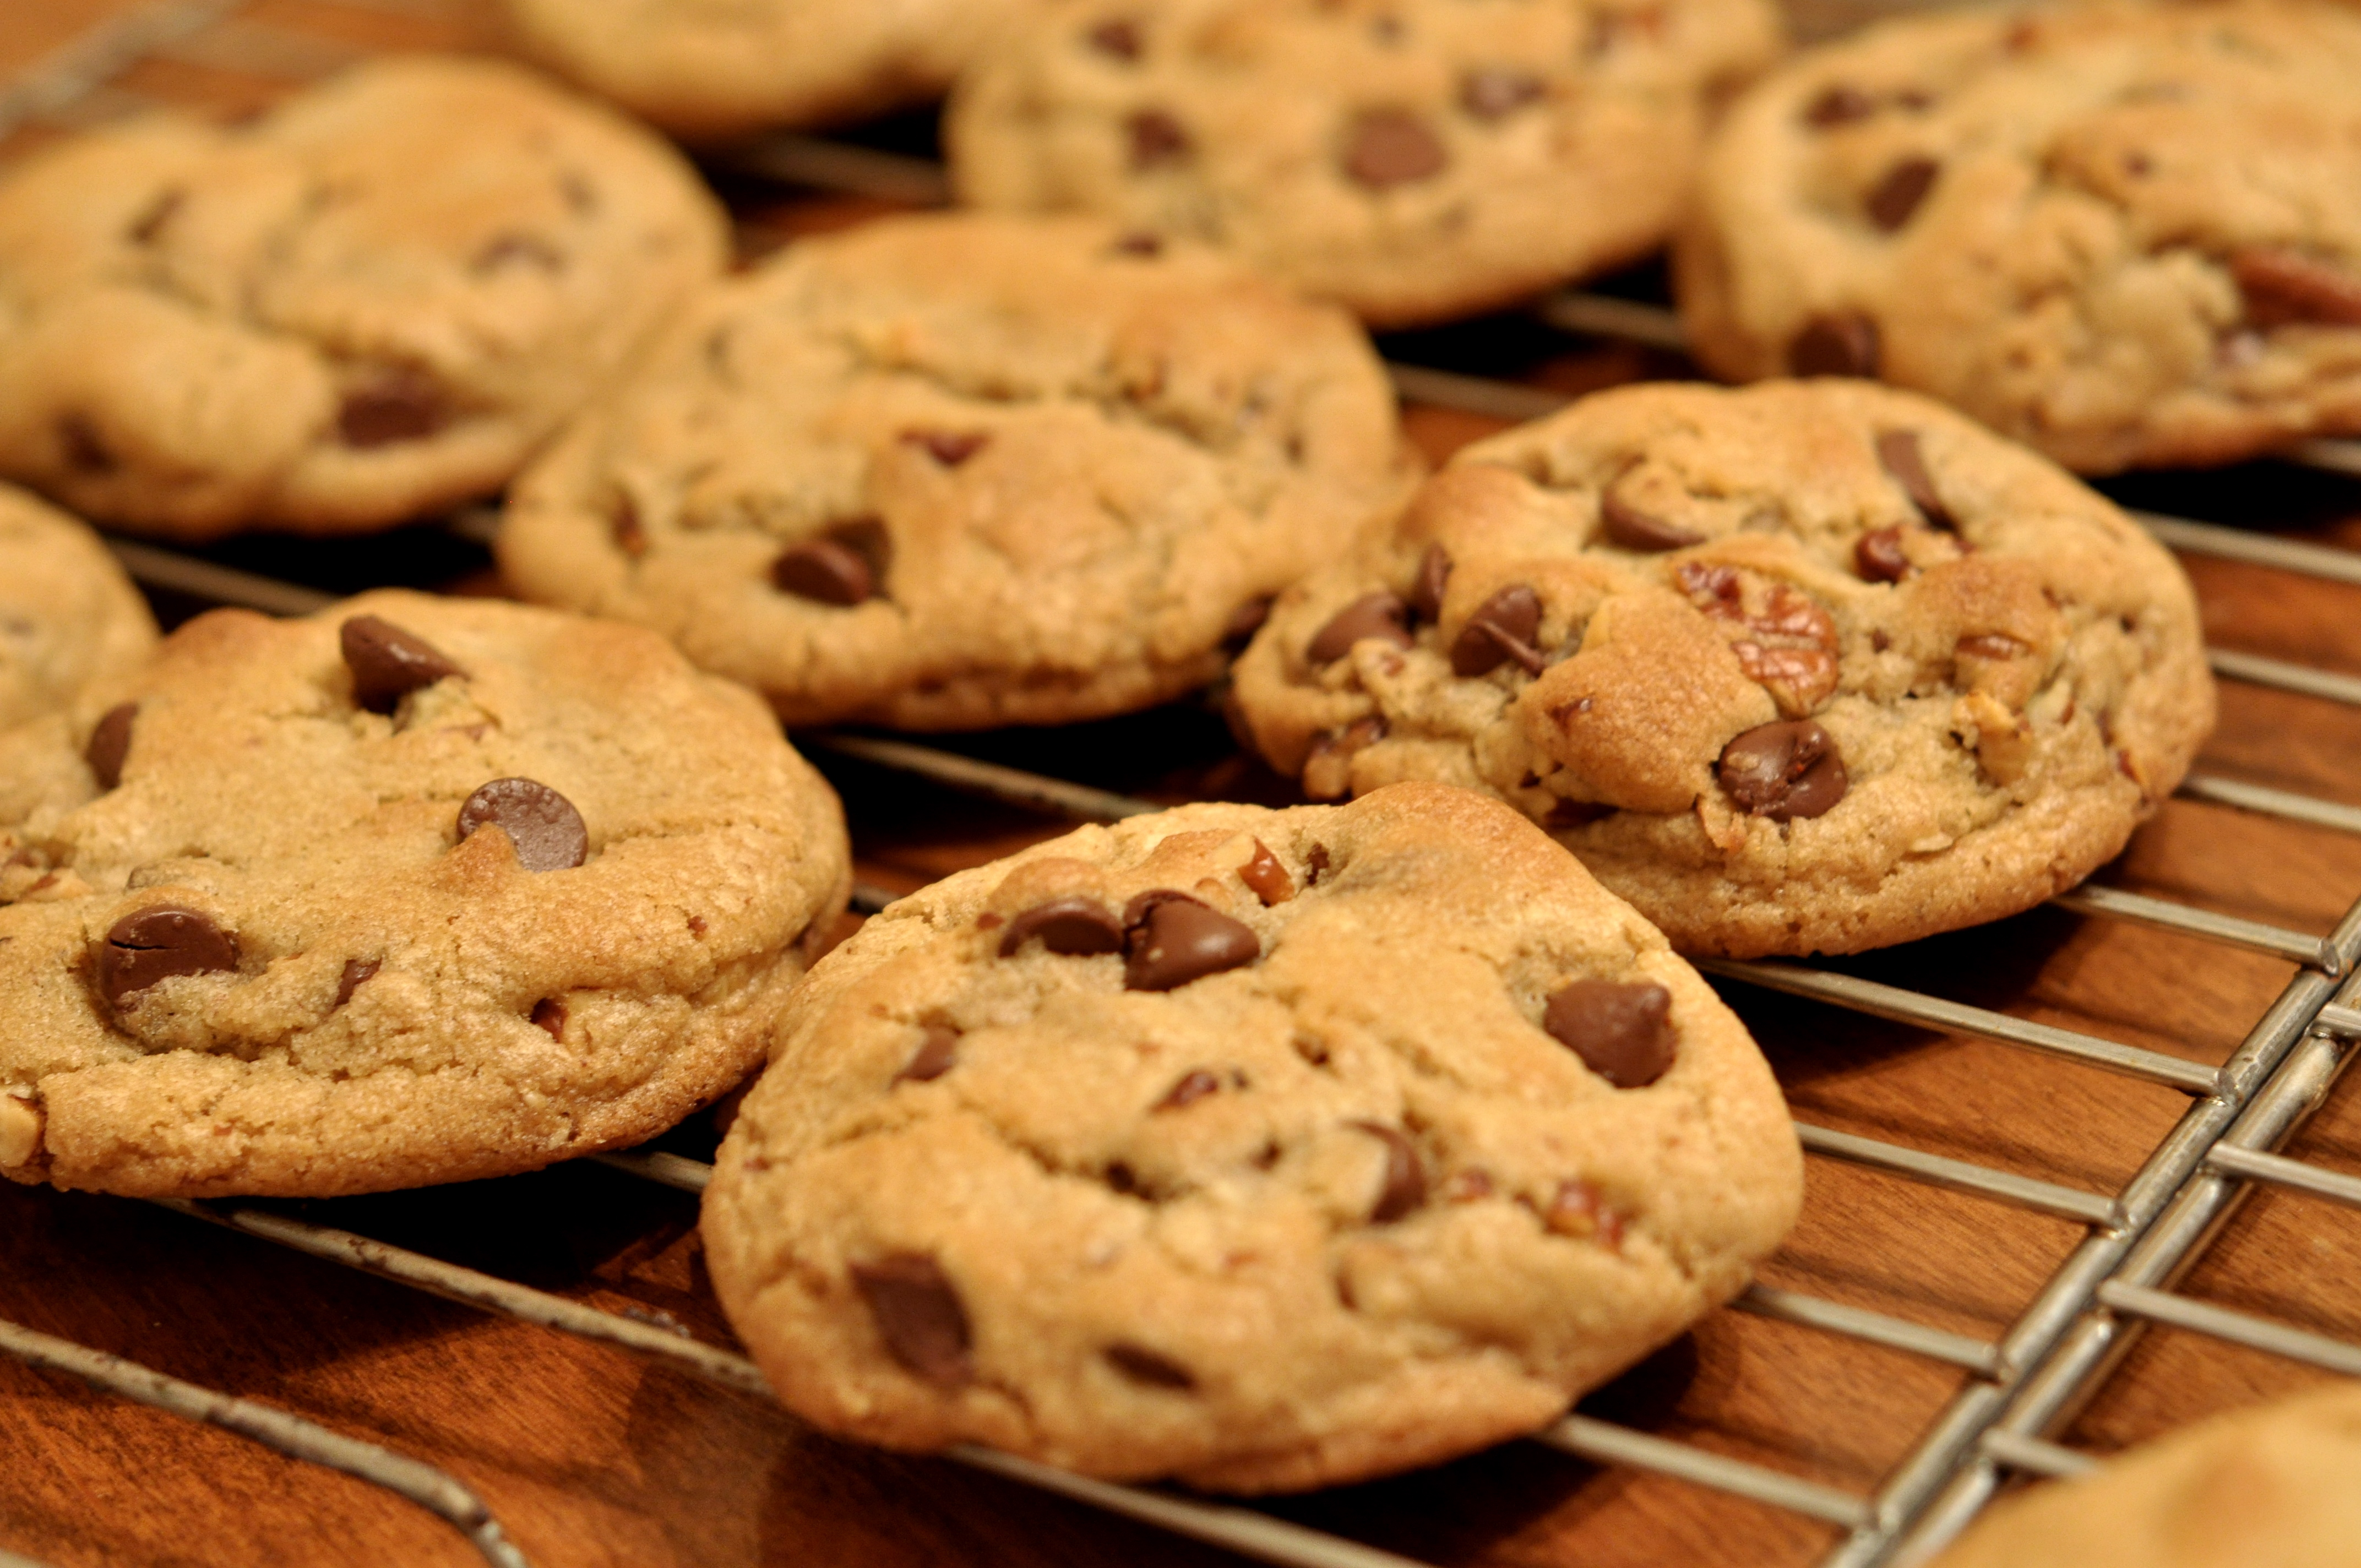
\includegraphics[width=.5\textwidth]{images/cookie}}

\def\questionD{-}
\def\answerD{-}

\def\questionE{-}
\def\answerE{-}

\def\questionF{-}
\def\answerF{-}

\def\questionG{-}
\def\answerG{-}

\def\questionH{-}
\def\answerH{-}

\def\questionI{-}
\def\answerI{-}

\def\questionJ{-}
\def\answerJ{-}

\generateQAs

%%%%%%%%%%%%%%%%%%%%%%%%%%%%%%%%%%%%%%%%%%%%%%%%%%%%%%%%%%%%%%%%%%%%%%%%%%%%%%%%%%%%%%%%%%%%%%%%%%%%%%%%%%%%%%%%%%%%%%%%
%%%%%%%%%%%%%%%%%%%%%%%%%%%%%%%%%%%%%%%%%%%%%%%%%%%%%%%%%%%%%%%%%%%%%%%%%%%%%%%%%%%%%%%%%%%%%%%%%%%%%%%%%%%%%%%%%%%%%%%%
%%%%%%%%%%%%%%%%%%%%%%%%%%%%%%%%%%%%%%%%%%%%%%%%%%%%%%%%%%%%%%%%%%%%%%%%%%%%%%%%%%%%%%%%%%%%%%%%%%%%%%%%%%%%%%%%%%%%%%%%

% \def\questionA{A}
% \def\answerA{A}

% \def\questionB{B}
% \def\answerB{B}

% \def\questionC{C}
% \def\answerC{C}

% \def\questionD{D}
% \def\answerD{D}

% \def\questionE{E}
% \def\answerE{E}

% \def\questionF{F}
% \def\answerF{F}

% \def\questionG{G}
% \def\answerG{G}

% \def\questionH{H}
% \def\answerH{H}

% \def\questionI{I}
% \def\answerI{I}

% \def\questionJ{J}
% \def\answerJ{J}

% \generateQAs

\end{document}